\documentclass[12pt,a4paper,oneside]{report}

\usepackage[utf8]{inputenc}
\usepackage[T1]{fontenc}
\usepackage[a4paper,left=2.5cm,right=1.5cm,top=2.5cm,bottom=2.5cm,headheight=20pt]{geometry}
\usepackage{amsmath}
\usepackage{graphicx}
\usepackage{float}
\usepackage{array}
\usepackage{booktabs}
\usepackage{longtable}
\usepackage{tabularx}
\usepackage{multirow}
\usepackage{enumitem}
\usepackage{xcolor}
\usepackage{tikz}
\usepackage{pdflscape}
\usepackage{caption}
\usepackage{hyperref}
\usepackage{setspace}
\usepackage{fancyhdr}

\usetikzlibrary{arrows.meta,positioning,shapes.geometric,fit,calc}
\graphicspath{{Images/}}
\setlength{\parindent}{0pt}
\setlength{\parskip}{1.1ex plus0.3ex minus0.2ex}
\setlist{itemsep=0.25ex, topsep=0.5ex}
\sloppy
\hypersetup{
    colorlinks=true,
    linkcolor=black,
    urlcolor=blue,
    citecolor=black,
    pdftitle={Smart Attendance Management System},
    pdfauthor={Project Team},
    pdfsubject={B.Tech Final Project Report},
    pdfkeywords={Smart Attendance, Face Recognition, MERN, FastAPI, MongoDB, Email Notification}
}

\newcommand{\projecttitle}{Smart Attendance Management System}
\newcommand{\productname}{MarkIn / SAMS}
\newcommand{\techstack}{React, Express, MongoDB, FastAPI and InsightFace}
\newcommand{\safepercent}{75\%}
\newcommand{\placeholder}[1]{\textbf{\textit{#1}}}

\pagestyle{fancy}
\fancyhead{}
\rhead{\thepage}
\lhead{\nouppercase{\leftmark}}

\begin{document}
\setstretch{1.2}
\pagenumbering{gobble}
\thispagestyle{empty}
\begin{titlepage}
\begin{center}
\vspace*{0.5cm}

{\LARGE \textbf{Smart Attendance Management System}\par}
\vspace{0.25cm}
{\Large \textbf{MarkIn / SAMS}\par}
\vspace{0.8cm}

\textbf{A Project Report Submitted\\
In Partial Fulfilment of the Requirements\\
for the Degree of}

\vspace{0.7cm}
{\textsc{\textbf{\large Bachelor of Technology}}\par}
\vspace{0.2cm}
\textbf{\large in}\par
\vspace{0.2cm}
{\textsc{\textbf{\large Computer Science \& Engineering}}\par}

\vspace{0.7cm}
{\large by\par}
\vspace{0.25cm}
{\textbf{\placeholder{Student Name 1} (Roll No. \placeholder{00000000000})}}\\
{\textbf{\placeholder{Student Name 2} (Roll No. \placeholder{00000000000})}}\\
{\textbf{\placeholder{Student Name 3} (Roll No. \placeholder{00000000000})}}\\

\vspace{0.85cm}
\textbf{Under the Guidance of}\\
{\textbf{\placeholder{Guide Name}}}\\

\vspace{1.1cm}

\includegraphics[width=0.2\linewidth]{ietlogo.png}
\vspace{0.8cm}

\textbf{\large Department of Computer Science and Engineering}\\
\vspace{0.12cm}
\textbf{\Large Institute of Engineering \& Technology}\\
\vspace{0.12cm}
{\large\textsc{\textbf{Dr. APJ Abdul Kalam Technical University, Uttar Pradesh}}}

\vfill
\textbf{\large \placeholder{May, 2026}}

\end{center}
\end{titlepage}
\clearpage


\pagenumbering{roman}
\chapter*{Certificate}
\addcontentsline{toc}{chapter}{Certificate}
This is to certify that the project report entitled \textbf{\projecttitle} submitted by \placeholder{Student Name 1 (Roll No.)}, \placeholder{Student Name 2 (Roll No.)} and \placeholder{Student Name 3 (Roll No.)} in partial fulfilment for the award of the degree of Bachelor of Technology in Computer Science \& Engineering is a record of the bonafide work carried out under the guidance of \placeholder{Guide Name}, Department of Computer Science and Engineering, Institute of Engineering \& Technology, Lucknow.

\vspace{1cm}
The project report has reached the standard required for submission. The work described in this report has not been submitted elsewhere for the award of any other degree or diploma to the best of our knowledge.

\vspace{2cm}
\begin{tabularx}{\textwidth}{X X}
\textbf{Date:} \placeholder{DD Month YYYY} & \textbf{Guide Signature:} \placeholder{Guide Name}\\
& Department of Computer Science and Engineering\\
& Institute of Engineering \& Technology, Lucknow
\end{tabularx}

\chapter*{Declaration}
\addcontentsline{toc}{chapter}{Declaration}
We hereby declare that this project report entitled \textbf{\projecttitle} is our own work carried out as part of the Bachelor of Technology final year project. The report explains the design, implementation, testing and evaluation of a smart attendance platform developed for students and teachers. Any external concepts, technologies and documentation referred to in the report have been acknowledged in the References section.

\vspace{2cm}
\begin{tabularx}{\textwidth}{X X X}
\placeholder{Student 1} & \placeholder{Student 2} & \placeholder{Student 3}\\
\placeholder{Roll No.} & \placeholder{Roll No.} & \placeholder{Roll No.}
\end{tabularx}

\chapter*{Acknowledgement}
\addcontentsline{toc}{chapter}{Acknowledgement}
We express our sincere gratitude to our project guide \placeholder{Guide Name} for valuable guidance, review and encouragement throughout this work. We also thank the Department of Computer Science and Engineering, Institute of Engineering \& Technology, Lucknow, for providing the academic environment and resources needed to complete the project. We are thankful to our teachers, classmates and family members for their support during requirement analysis, development, testing and documentation.

\chapter*{Abstract}
\addcontentsline{toc}{chapter}{Abstract}
The \projecttitle{} is a full-stack attendance management platform designed to reduce manual work, improve transparency and support academic decision-making. The system provides role-based dashboards for students and teachers, class creation and joining, face enrollment, AI-assisted classroom photo attendance, QR attendance, manual attendance, attendance analytics, leave proof upload, exam eligibility planning, email notifications and report export. The backend is built with Express and MongoDB, the frontend is built with React, and a separate FastAPI AI service performs face detection and recognition using InsightFace model packs such as Antelopev2 and Buffalo\_L.

Unlike a simple attendance register, the system follows a review-first workflow. When a teacher captures classroom photos, the AI service suggests present and absent students. The result is stored in a Today Attendance Data draft, absentees are notified by email, and the teacher can correct the list before final submission. This reduces false marking and gives students a chance to report mistakes. The project also includes email OTP verification, password reset, profile email verification, leave approval/rejection emails, exam attendance warnings and class cancellation notices. This report explains the complete project from beginner level: problem background, requirements, system design, database structure, workflows, implementation, testing, results, limitations and future scope.

\tableofcontents
\listoffigures
\listoftables
\clearpage
\pagenumbering{arabic}

\chapter{Introduction}
\label{ch:introduction}
\lhead{Chapter 1. \emph{Introduction}}

\section{Project Overview}
Attendance is one of the most common administrative activities in schools, colleges and training institutions. In many classrooms it is still handled by calling names, signing registers or manually entering presence into a spreadsheet. These methods are simple, but they become slow and unreliable when the number of students and classes increases. A teacher may spend several minutes marking attendance, students may be marked incorrectly, and the attendance percentage may not be visible to students until it is too late to recover.

The \projecttitle{} is designed as a modern solution to this problem. It combines a web application, a backend API, a database and an artificial intelligence service. Teachers can create classes, add or invite students, run attendance using classroom photographs, verify results, manage students, schedule exams and review leave requests. Students can join classes, enroll their face profile, view attendance analytics, upload leave proof, check exam eligibility and receive notifications. The system is not only an attendance marker; it is an academic support platform that explains what the attendance data means.

The product name used in the user interface is \productname. SAMS stands for Smart Attendance Management System. The word MarkIn represents the idea of marking attendance in a smarter and safer way. The project is implemented as a three-service architecture: React frontend, Express backend and FastAPI AI service. MongoDB is used for persistent storage, and the AI service uses face detection and recognition models to support photo-based attendance.

\section{Motivation}
The main motivation behind this project is to make attendance more accurate, transparent and useful. Traditional attendance systems usually solve only one task: recording present or absent. In practice, an institution needs much more. Teachers need a clean roster and a safe way to correct AI mistakes. Students need to know which class is weak, how many classes they must attend before an exam and whether leave proof was approved. Administrators need records that can be audited and exported.

The project therefore focuses on four ideas:
\begin{enumerate}[label=\arabic*.]
    \item \textbf{Reduce teacher workload:} Camera-based attendance, QR attendance and manual controls reduce repetitive work.
    \item \textbf{Protect correctness:} AI suggestions are not blindly finalized; a teacher reviews Today Attendance Data before submission.
    \item \textbf{Inform students early:} Low attendance, absence, leave status and exam eligibility are communicated through dashboards and email.
    \item \textbf{Keep data useful:} Attendance is converted into analytics, recovery guidance, class summaries and CSV reports.
\end{enumerate}

\section{Problem Statement}
Educational institutions require a reliable attendance management system that can record attendance efficiently, reduce manual errors, support verification, notify students about important attendance events and provide meaningful analytics. Existing manual or semi-digital methods are often slow, fragmented and reactive. They do not provide real-time correction workflows, AI-assisted classroom verification, leave proof handling, exam eligibility planning or email-based communication in one integrated product.

The problem can be stated as follows:

\begin{quote}
To design and implement a full-stack Smart Attendance Management System that allows teachers and students to manage attendance, class activities, AI-assisted verification, leave documentation, exam eligibility and notifications through a secure and user-friendly web platform.
\end{quote}

\section{Objectives}
The objectives of the project are:
\begin{itemize}
    \item To provide separate student and teacher dashboards with role-based access.
    \item To allow teachers to create classes and students to join using class codes.
    \item To allow students to enroll face profiles for classroom photo attendance.
    \item To implement AI-assisted recognition using a separate FastAPI service.
    \item To create a review-first attendance workflow where teachers verify results before final submission.
    \item To send email notifications for verification, password reset, absence, leave status, exam warnings and class cancellation.
    \item To provide student analytics such as total classes, present count, absent count, percentage and recovery guidance.
    \item To support leave or medical proof upload with teacher approval/rejection.
    \item To support exam scheduling and attendance eligibility calculation.
    \item To keep the architecture modular, maintainable and scalable.
\end{itemize}

\section{Scope of the Project}
The current project scope includes frontend user experience, backend business rules, MongoDB persistence, AI-service integration and email notification workflows. The system supports real classroom workflows such as class creation, joining, attendance capture, draft review, final submission, QR attendance, manual attendance, leave proof, assignments, discussion, notes, exams and analytics.

The project does not claim to replace institutional ERP systems completely. Instead, it focuses on attendance-centered academic operations. It can later integrate with ERP, biometric hardware, institutional SSO, payment systems or official exam portals if required.

\section{Users of the System}
\begin{table}[H]
\centering
\caption{Primary users of the system}
\label{tab:users}
\begin{tabularx}{\textwidth}{p{3.2cm}X}
\toprule
\textbf{User Type} & \textbf{Purpose in System}\\
\midrule
Student & Joins classes, enrolls face profile, views attendance, checks exam eligibility, receives notifications and submits leave proof.\\
Teacher & Creates classes, manages rosters, runs attendance, corrects Today Attendance Data, finalizes attendance, reviews leave requests and schedules exams.\\
AI Service & Performs face detection, embedding generation, roster matching and attendance session analysis.\\
Backend Service & Owns authentication, authorization, MongoDB access, email delivery, attendance rules and API orchestration.\\
\bottomrule
\end{tabularx}
\end{table}

\section{Why the Project is Useful}
The usefulness of the project is visible from both student and teacher perspectives. A student does not need to guess whether attendance is safe for exams. The dashboard shows joined classes, attendance percentages, present/absent counts, upcoming exams and minimum classes to attend. A teacher does not need to manually call every student name when a clear classroom photo is available. The AI service suggests attendance, but final control remains with the teacher.

The system also solves a common communication gap. If a student is marked absent from photo attendance, the student receives an email immediately after the draft is created. If the student believes the result is wrong, the teacher can correct the draft before final submission. This small workflow makes the system more trustworthy than a direct AI auto-submit model.

\section{Report Organization}
This report is organized to help a beginner understand the project step by step. Chapter 2 discusses existing systems and related concepts. Chapter 3 explains requirements. Chapter 4 describes architecture and design. Chapter 5 explains implementation. Chapter 6 explains features and working flows. Chapter 7 presents testing and results. Chapter 8 concludes the work with limitations and future scope. The appendix contains route summaries, setup guidance and additional reference material.

\chapter{Literature Review and Existing Systems}
\label{ch:related}
\lhead{Chapter 2. \emph{Literature Review and Existing Systems}}

\section{Background}
Attendance management has evolved from paper registers to digital portals and biometric systems. The earliest method is the manual register, where the teacher calls student names and marks presence. Later, spreadsheet-based records and ERP portals reduced paper usage but still required manual entry. Biometric devices such as fingerprint scanners improved automation but require fixed hardware and may not be suitable for every classroom. QR-based systems are easy to deploy but can be misused if students share codes.

Recent systems use face recognition to identify students from images or video. This approach can reduce teacher workload, but it must be designed carefully. Classroom photographs may contain partial faces, different angles, low lighting, occlusions and multiple students. An attendance system should therefore avoid blind automatic finalization. The safest approach is assisted intelligence: AI suggests, teacher verifies and the final record is written only after review.

\section{Manual Attendance Systems}
Manual systems remain common because they are easy to understand and require no technical infrastructure. However, they are time-consuming and error-prone. A teacher may accidentally mark a student absent, and students may not learn about low attendance until exam time. Manual systems also make reporting difficult because the data is scattered across notebooks or spreadsheets.

\begin{table}[H]
\centering
\caption{Limitations of manual attendance}
\label{tab:manual-limitations}
\begin{tabularx}{\textwidth}{p{4cm}X}
\toprule
\textbf{Limitation} & \textbf{Impact}\\
\midrule
Time consumption & Classroom teaching time is reduced because attendance must be called manually.\\
Human error & Wrong marking can occur due to missed names, late entries or register mistakes.\\
Delayed visibility & Students may not know exact attendance percentage until records are calculated.\\
Weak reporting & Manual data is difficult to analyze, export or connect with exam eligibility rules.\\
No automatic notification & Students and parents are not informed immediately about absence or risk.\\
\bottomrule
\end{tabularx}
\end{table}

\section{Digital ERP Attendance Systems}
Many institutions use ERP portals where teachers enter attendance into a web form. Such systems improve record storage and calculation but often do not reduce the teacher's marking effort. They may also be generic and not optimized for classroom realities such as face enrollment, leave proof, AI review, student-side recovery planning or exam eligibility.

The proposed system keeps the useful parts of ERP systems, such as persistent records and role-based access, but adds attendance-specific workflows. For example, the teacher class workspace includes AI photo attendance, Today Attendance Data, manual attendance, QR attendance, CSV download, student details, leave requests and exam setup.

\section{Biometric Attendance Systems}
Fingerprint or RFID-based attendance systems are common in offices and some institutions. They can verify presence using hardware devices. However, classroom use may face practical problems: device cost, queues, hygiene concerns, hardware maintenance, and lack of flexibility when classes move between rooms. Face recognition from classroom photos is more flexible because it can use a teacher's phone or uploaded images.

At the same time, face recognition is not perfect. It must be combined with quality checks, confidence scores and teacher review. SAMS therefore treats AI recognition as a decision-support component, not a final authority.

\section{QR Attendance Systems}
QR attendance is popular because it is simple. A teacher displays a QR code, and students scan it to mark themselves present. The main advantage is speed. The main risk is misuse: a student can share the QR link with someone outside the room unless extra controls are used. In SAMS, QR attendance is included as an alternative attendance method, but AI photo attendance and manual teacher control remain available.

\section{Face Recognition Concepts}
Face recognition systems generally involve four steps:
\begin{enumerate}[label=\arabic*.]
    \item Detect faces in an image.
    \item Align or normalize detected faces.
    \item Convert each face into a numerical embedding.
    \item Compare embeddings with stored face profiles.
\end{enumerate}

The AI service in this project uses InsightFace model packs. Detection is performed by models such as SCRFD or RetinaFace, and recognition uses ArcFace-style embeddings. A face embedding is a vector representation of a face. If two embeddings are close by cosine similarity, they are likely to belong to the same person. The system also compares against the second-best match to avoid accepting ambiguous results.

\section{Related Technology Stack}
The project uses a MERN-style web architecture combined with a Python AI service. This split is useful because web business rules and machine learning workloads have different needs. React is suitable for interactive dashboards. Express is suitable for REST APIs and orchestration. MongoDB is suitable for flexible document storage. FastAPI is suitable for model-serving endpoints and Python ML libraries.

\begin{table}[H]
\centering
\caption{Technology stack overview}
\label{tab:stack}
\begin{tabularx}{\textwidth}{p{3.2cm}p{4cm}X}
\toprule
\textbf{Layer} & \textbf{Technology} & \textbf{Reason}\\
\midrule
Frontend & React, Parcel, JavaScript & Component-based dashboards, fast development and single-page routing.\\
Backend & Node.js, Express & REST API, authentication, classroom rules and email orchestration.\\
Database & MongoDB, Mongoose & Flexible documents for classes, users, records, leave requests and email logs.\\
AI Service & FastAPI, Python & Model serving, image processing and machine learning workflows.\\
Face Models & InsightFace, ArcFace, SCRFD & Real face detection and recognition model support.\\
Email & Nodemailer, Gmail SMTP & OTP, password reset, absence and academic notifications.\\
\bottomrule
\end{tabularx}
\end{table}

\section{Gap in Existing Solutions}
Most attendance systems focus on marking presence. Fewer systems combine attendance marking with student learning support. The important gap is not just recording who was absent, but helping the student act on it. SAMS addresses this gap with:
\begin{itemize}
    \item student analytics and per-class detail pages;
    \item exam eligibility warnings and calculator;
    \item leave/medical proof upload;
    \item email alerts and notification center;
    \item teacher-controlled AI attendance draft review;
    \item class notes, assignments and discussion.
\end{itemize}

\section{Proposed Direction}
The proposed direction is a review-first smart attendance platform. AI is used to speed up attendance recognition, but the teacher remains responsible for final submission. This balances automation and accountability. The system also turns attendance data into useful academic guidance rather than treating it as a hidden administrative record.

\chapter{Requirement Analysis}
\label{chap:requirements}

Requirement analysis explains what the system must do, who will use it, which data it must handle, and what quality conditions must be satisfied. For \productname{}, the requirements were derived from the practical problems faced in daily attendance work: teachers need faster marking, students need transparency, and administrators need dependable records. The system therefore combines attendance capture, verification, analytics, document proof, exam eligibility and email communication into one connected workflow.

\section{Stakeholders}

The project has two primary user groups and a few supporting stakeholders. A teacher operates classes, attendance sessions, leave approvals and exam rules. A student joins classes, checks attendance, submits documents and receives alerts. The department or institute can use the stored data for records, compliance and reports. Parents may optionally receive absence alerts when the student profile contains a parent email address.

\begin{table}[H]
\centering
\caption{Stakeholders and their expectations}
\label{tab:stakeholders}
\begin{tabularx}{\textwidth}{p{3cm} X X}
\toprule
\textbf{Stakeholder} & \textbf{Main expectation} & \textbf{How SAMS supports it}\\
\midrule
Student & Clear attendance status, class-wise records, exam eligibility, proof submission and alerts. & Student dashboard, class detail pages, attendance calculator, leave proof upload, notification page and email alerts.\\
Teacher & Fast attendance capture, reliable correction, class management and student analytics. & Teacher dashboard, AI photo attendance, Today Attendance Data draft, manual edits, QR attendance, leave review and exam setup.\\
Department & Consistent attendance records and reduced manual paperwork. & MongoDB-backed records, final attendance submission, export-ready summaries and audit-friendly email logs.\\
Parent or guardian & Optional awareness when a student is absent. & Optional parent email on the student profile for absent notifications.\\
System maintainer & Modular codebase and simple deployment. & Separate frontend, backend and AI service with environment-based configuration.\\
\bottomrule
\end{tabularx}
\end{table}

\section{Functional Requirements}

Functional requirements describe the visible actions supported by the application. The first major requirement is authentication. Students and teachers should be able to register, verify their email using an OTP, log in, update profile details and reset forgotten passwords. The system must not treat an unverified account as fully active because email is used for important academic notifications.

The second requirement is class management. A teacher should be able to create a class with subject name, subject code, section, semester, academic year, room and weekly schedule. Students should be able to join a class through a join code or join link. The teacher should be able to view the roster and add, update or remove students when needed.

The third requirement is attendance capture. The system should allow manual attendance, QR attendance and AI-assisted photo attendance. Manual attendance is useful when a teacher wants direct control. QR attendance is useful when students physically present in class can scan a session code. AI-assisted photo attendance is useful when the teacher wants to take classroom photos and let the system identify likely present students.

The fourth requirement is review before finalization. Photo attendance cannot be considered perfect because classroom lighting, camera angle, occlusion and missing face enrollment can affect recognition. Therefore, AI results must first go to a draft area called Today Attendance Data. The teacher can add or remove students from this draft. Absentees are notified early so that a mistaken absence can be reported before final submission. If the teacher does not finalize manually, the backend scheduler can finalize eligible drafts after the configured delay.

The fifth requirement is student usefulness. A student dashboard should not simply show a percentage. It should show total classes, present count, absent count, class-wise status, upcoming exams, safe attendance information, notifications and navigation to separate class pages. Each class page should provide schedule, recent attendance, leave proof submission and useful context for improving attendance.

The sixth requirement is academic communication. The backend must send professional emails for signup verification, welcome message, password reset, profile email verification, leave approval or rejection, absent notification, exam attendance warning and class cancellation or rescheduling. The email module should be modular, retry failed delivery and store delivery status without exposing SMTP secrets.

\begin{longtable}{p{3.2cm} p{4.6cm} p{5.8cm}}
\caption{Functional requirement summary}
\label{tab:functional-reqs}\\
\toprule
\textbf{Module} & \textbf{Requirement} & \textbf{Expected behaviour}\\
\midrule
\endfirsthead
\toprule
\textbf{Module} & \textbf{Requirement} & \textbf{Expected behaviour}\\
\midrule
\endhead
Authentication & Email verified registration & User enters registration details, receives OTP, verifies email and then receives a welcome email.\\
Authentication & Forgot password & User requests reset, receives OTP or reset token, and can set a new password before expiry.\\
Profile & Email update & User submits new email, verifies OTP and only then the profile email is changed.\\
Classroom & Teacher creates class & Teacher defines subject, code, section, schedule and metadata. System generates join code.\\
Classroom & Student joins class & Student submits join code and becomes part of the class roster.\\
Attendance & Manual marking & Teacher can directly mark present, absent, late, excused or cancelled records.\\
Attendance & QR marking & Teacher creates a QR session; students scan to mark attendance within the allowed window.\\
Attendance & Photo marking & Teacher uploads classroom photo; backend sends it to AI service; suggested attendance is stored as a draft.\\
Draft review & Today Attendance Data & Teacher sees present and absent names, corrects the draft and finalizes it.\\
Leave proof & Student upload & Student submits reason, absence date and image or PDF proof from the class detail page.\\
Leave review & Teacher decision & Teacher previews files online, approves or rejects, and student receives email.\\
Exam planning & Teacher exam setup & Teacher sets exam date and required attendance percentage.\\
Exam planning & Student eligibility & Student sees eligibility, minimum classes to attend and warnings when below threshold.\\
Notifications & Dashboard alerts & Important alerts appear under the student notification bell and notification page.\\
Email & Delivery logging & Each email event is queued, retried and written to delivery logs with safe metadata.\\
\bottomrule
\end{longtable}

\section{Non-Functional Requirements}

Non-functional requirements describe the quality of the system rather than a single button or page. In an attendance system these qualities are important because incorrect records can directly affect student eligibility. The system must be reliable, understandable, responsive, secure and maintainable.

\begin{table}[H]
\centering
\caption{Non-functional requirements}
\label{tab:nonfunctional}
\begin{tabularx}{\textwidth}{p{3.5cm} X}
\toprule
\textbf{Quality attribute} & \textbf{Requirement for this project}\\
\midrule
Usability & Dashboards should show the most useful information first and should avoid confusing students with raw data only.\\
Accuracy & AI attendance should be treated as an assistive result, not an unquestioned final record. Teacher review remains part of the workflow.\\
Security & Passwords, email OTPs, SMTP credentials and database connection strings must not be exposed in frontend code or reports.\\
Performance & Dashboard APIs should return summarized data so that the frontend can render quickly without doing heavy calculations.\\
Scalability & Email sending should use a queue and limited concurrency so bulk class notifications do not block normal API responses.\\
Maintainability & Frontend, backend and AI logic should remain separated so each service can evolve independently.\\
Observability & Health and email status endpoints should show safe operational state without revealing secrets.\\
Portability & The app should run locally through workspace scripts and should support Docker-based deployment.\\
\bottomrule
\end{tabularx}
\end{table}

\section{User Roles and Permissions}

Role separation is necessary because students and teachers perform different actions. The student should not be able to finalize attendance or approve leave. The teacher should not need direct database access. The backend API is the control point for enforcing these actions.

\begin{table}[H]
\centering
\caption{User roles and permissions}
\label{tab:roles}
\begin{tabularx}{\textwidth}{p{3cm} X X}
\toprule
\textbf{Action} & \textbf{Student} & \textbf{Teacher}\\
\midrule
Register and verify email & Allowed & Allowed\\
Log in and update profile & Allowed & Allowed\\
Create class & Not allowed & Allowed\\
Join class & Allowed & Not required\\
View own attendance & Allowed & Can view class attendance\\
View all students in a class & Not allowed & Allowed for own classes\\
Submit leave proof & Allowed for own class membership & Not applicable\\
Preview leave proof & Own submissions only & Allowed for students in own class\\
Approve or reject leave & Not allowed & Allowed\\
Set exam date and eligibility threshold & Not allowed & Allowed\\
Use attendance calculator & Allowed & Can interpret class-level analytics\\
Create attendance draft & Not allowed & Allowed\\
Edit and finalize Today Attendance Data & Not allowed & Allowed\\
\bottomrule
\end{tabularx}
\end{table}

\section{Use Case View}

A beginner can understand the system through use cases. A use case is a user goal written from the user's perspective. For example, ``student checks exam eligibility'' is a use case. It is not just a page; it includes input data, processing and result.

\begin{figure}[H]
\centering
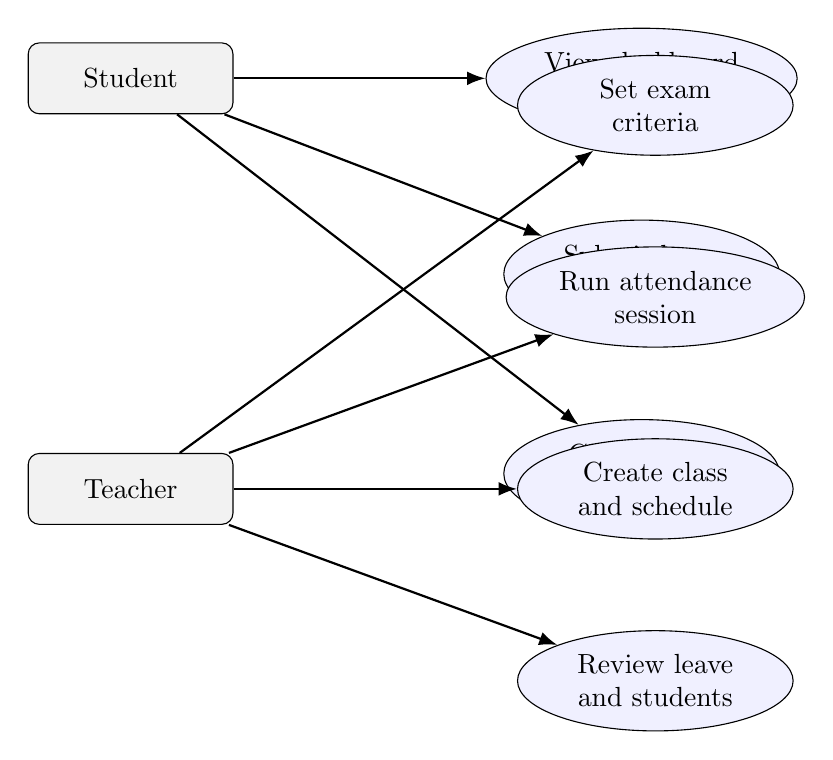
\begin{tikzpicture}[
actor/.style={draw, rounded corners, minimum width=2.6cm, minimum height=0.9cm, fill=gray!10},
case/.style={draw, ellipse, align=center, minimum width=3.5cm, minimum height=1cm, fill=blue!6},
line/.style={-Latex, thick}
]
\node[actor] (student) {Student};
\node[actor, below=4.3cm of student] (teacher) {Teacher};
\node[case, right=3.2cm of student] (dash) {View dashboard\\and notifications};
\node[case, below=1.15cm of dash] (leave) {Submit leave\\proof};
\node[case, below=1.15cm of leave] (calc) {Check exam\\eligibility};
\node[case, right=3.6cm of teacher] (class) {Create class\\and schedule};
\node[case, above=1.15cm of class] (att) {Run attendance\\session};
\node[case, below=1.15cm of class] (review) {Review leave\\and students};
\node[case, above=1.15cm of att] (exam) {Set exam\\criteria};
\draw[line] (student) -- (dash);
\draw[line] (student) -- (leave);
\draw[line] (student) -- (calc);
\draw[line] (teacher) -- (class);
\draw[line] (teacher) -- (att);
\draw[line] (teacher) -- (review);
\draw[line] (teacher) -- (exam);
\end{tikzpicture}
\caption{High-level user role use cases}
\label{fig:usecases}
\end{figure}

\section{Data Requirements}

The system requires structured data about users, classes, attendance, face enrollment, leave requests, exams and email events. MongoDB is a suitable choice because class and attendance documents may contain nested schedule slots, attachment metadata and draft records. The backend still defines schemas using Mongoose so the application has validation and consistent field names.

\begin{table}[H]
\centering
\caption{Important data required by SAMS}
\label{tab:data-requirements}
\begin{tabularx}{\textwidth}{p{3.5cm} X}
\toprule
\textbf{Data item} & \textbf{Purpose}\\
\midrule
User profile & Stores role, user id, name, email, verification state, optional parent email and profile metadata.\\
Classroom & Stores teacher ownership, subject information, section, room, schedule and join code.\\
Class membership & Connects a student to a class and supports roster analytics.\\
Face profile & Stores enrollment state and face embeddings or metadata needed by the AI-backed workflow.\\
Attendance record & Stores final attendance decisions with status, date, class and source.\\
Attendance draft & Stores temporary Today Attendance Data before final submission.\\
Leave request & Stores absence date, reason, request type, attachments and review decision.\\
Class exam & Stores exam date, required attendance percentage and teacher notes.\\
Email delivery log & Stores delivery status, template name, recipient metadata and error details if sending fails.\\
\bottomrule
\end{tabularx}
\end{table}

\section{Input and Output Requirements}

Inputs must be simple enough for a normal college user. A teacher should only need class details, attendance photos, QR controls or manual status selections. A student should only need join code, profile details, absence reason, proof files and optional calculator inputs. The backend should validate these inputs before storing them.

The outputs should be actionable. Instead of only showing raw attendance records, the student dashboard should answer questions such as: How many classes have I joined? Which class is risky? How many total sessions were held? How many were present or absent? Am I eligible for the next exam? How many future classes should I attend to be safe? The teacher dashboard should answer questions such as: Which classes need action today? Which students are below range? Which leave requests are pending? Which attendance drafts still require final submission?

\section{Constraints and Assumptions}

The project assumes a college environment where classes are organized by teacher, subject and section. The system assumes that students and teachers have email access because verification and alerts are part of the workflow. It also assumes that the teacher remains responsible for final attendance accuracy because computer vision cannot be perfect under all classroom conditions.

The major technical constraints are camera quality, lighting conditions, network availability and the availability of AI model files. If the AI service is unavailable, manual or QR attendance can still support the academic workflow. If email delivery fails, the backend records the failure and can be configured with retries. If a student has not completed face enrollment, the system warns the student and the teacher can rely on other attendance methods.

\section{Requirement Traceability}

Requirement traceability helps connect features to project modules. This makes testing easier because each requirement can be mapped to a backend service and a frontend page.

\begin{longtable}{p{3.4cm} p{4.4cm} p{5.8cm}}
\caption{Requirement traceability matrix}
\label{tab:req-traceability}\\
\toprule
\textbf{Requirement} & \textbf{Backend area} & \textbf{Frontend area}\\
\midrule
\endfirsthead
\toprule
\textbf{Requirement} & \textbf{Backend area} & \textbf{Frontend area}\\
\midrule
\endhead
Email verification & Auth and email OTP services & Signup and verification screens\\
Student dashboard analytics & Student dashboard service and attendance analytics service & Student dashboard, notification page and class detail page\\
Teacher dashboard analytics & Teacher dashboard service and classroom services & Teacher dashboard and class students page\\
Face enrollment & Face profile service and AI service bridge & Student face enrollment page\\
Photo attendance & Attendance service, teacher classroom controller and AI gateway & Teacher attendance workspace\\
Today Attendance Data & Attendance draft model, scheduler and finalize endpoints & Teacher draft review section\\
Leave proof & Leave request service, attachment metadata and email notification service & Student class detail and teacher student detail page\\
Exam eligibility & Exam schedule service and attendance analytics & Upcoming exams section and calculator page\\
Notifications & Dashboard services and student notification builder & Bell icon and separate notification view\\
Email status & Email service and delivery logs & Email setup or test/status view\\
\bottomrule
\end{longtable}

This chapter defined the expectations of the system. The next chapter converts these requirements into an architecture and design that explains how the frontend, backend, database and AI service work together.

\chapter{System Design and Architecture}
\label{chap:architecture}

System design explains how the requirements are divided into cooperating parts. \productname{} follows a three-service architecture: a React frontend for user interaction, an Express backend for business rules and persistence, and a FastAPI AI service for face recognition. MongoDB stores the application data. This separation keeps the browser simple, keeps security-sensitive work inside the backend, and keeps machine learning code independent from normal web application code.

\section{Architectural Principles}

The design follows five practical principles. First, the backend is the source of truth. The frontend can display data and collect input, but it should not decide final attendance rules or directly contact the AI service. Second, AI should assist rather than replace teacher review. Third, every important academic event should be traceable: attendance finalization, leave approval, email delivery and exam eligibility are represented in backend records. Fourth, sensitive configuration must stay in environment variables and must never be included in source reports. Fifth, dashboards should present summarized information because students and teachers need decisions, not only raw tables.

\section{Overall Architecture}

Figure~\ref{fig:repo-architecture} shows the system architecture used by the project. The browser communicates only with the backend REST API. The backend validates requests, reads or writes MongoDB documents, sends email through SMTP and forwards recognition jobs to the AI service. The AI service loads face detection and recognition models and returns structured results.

\begin{figure}[H]
\centering
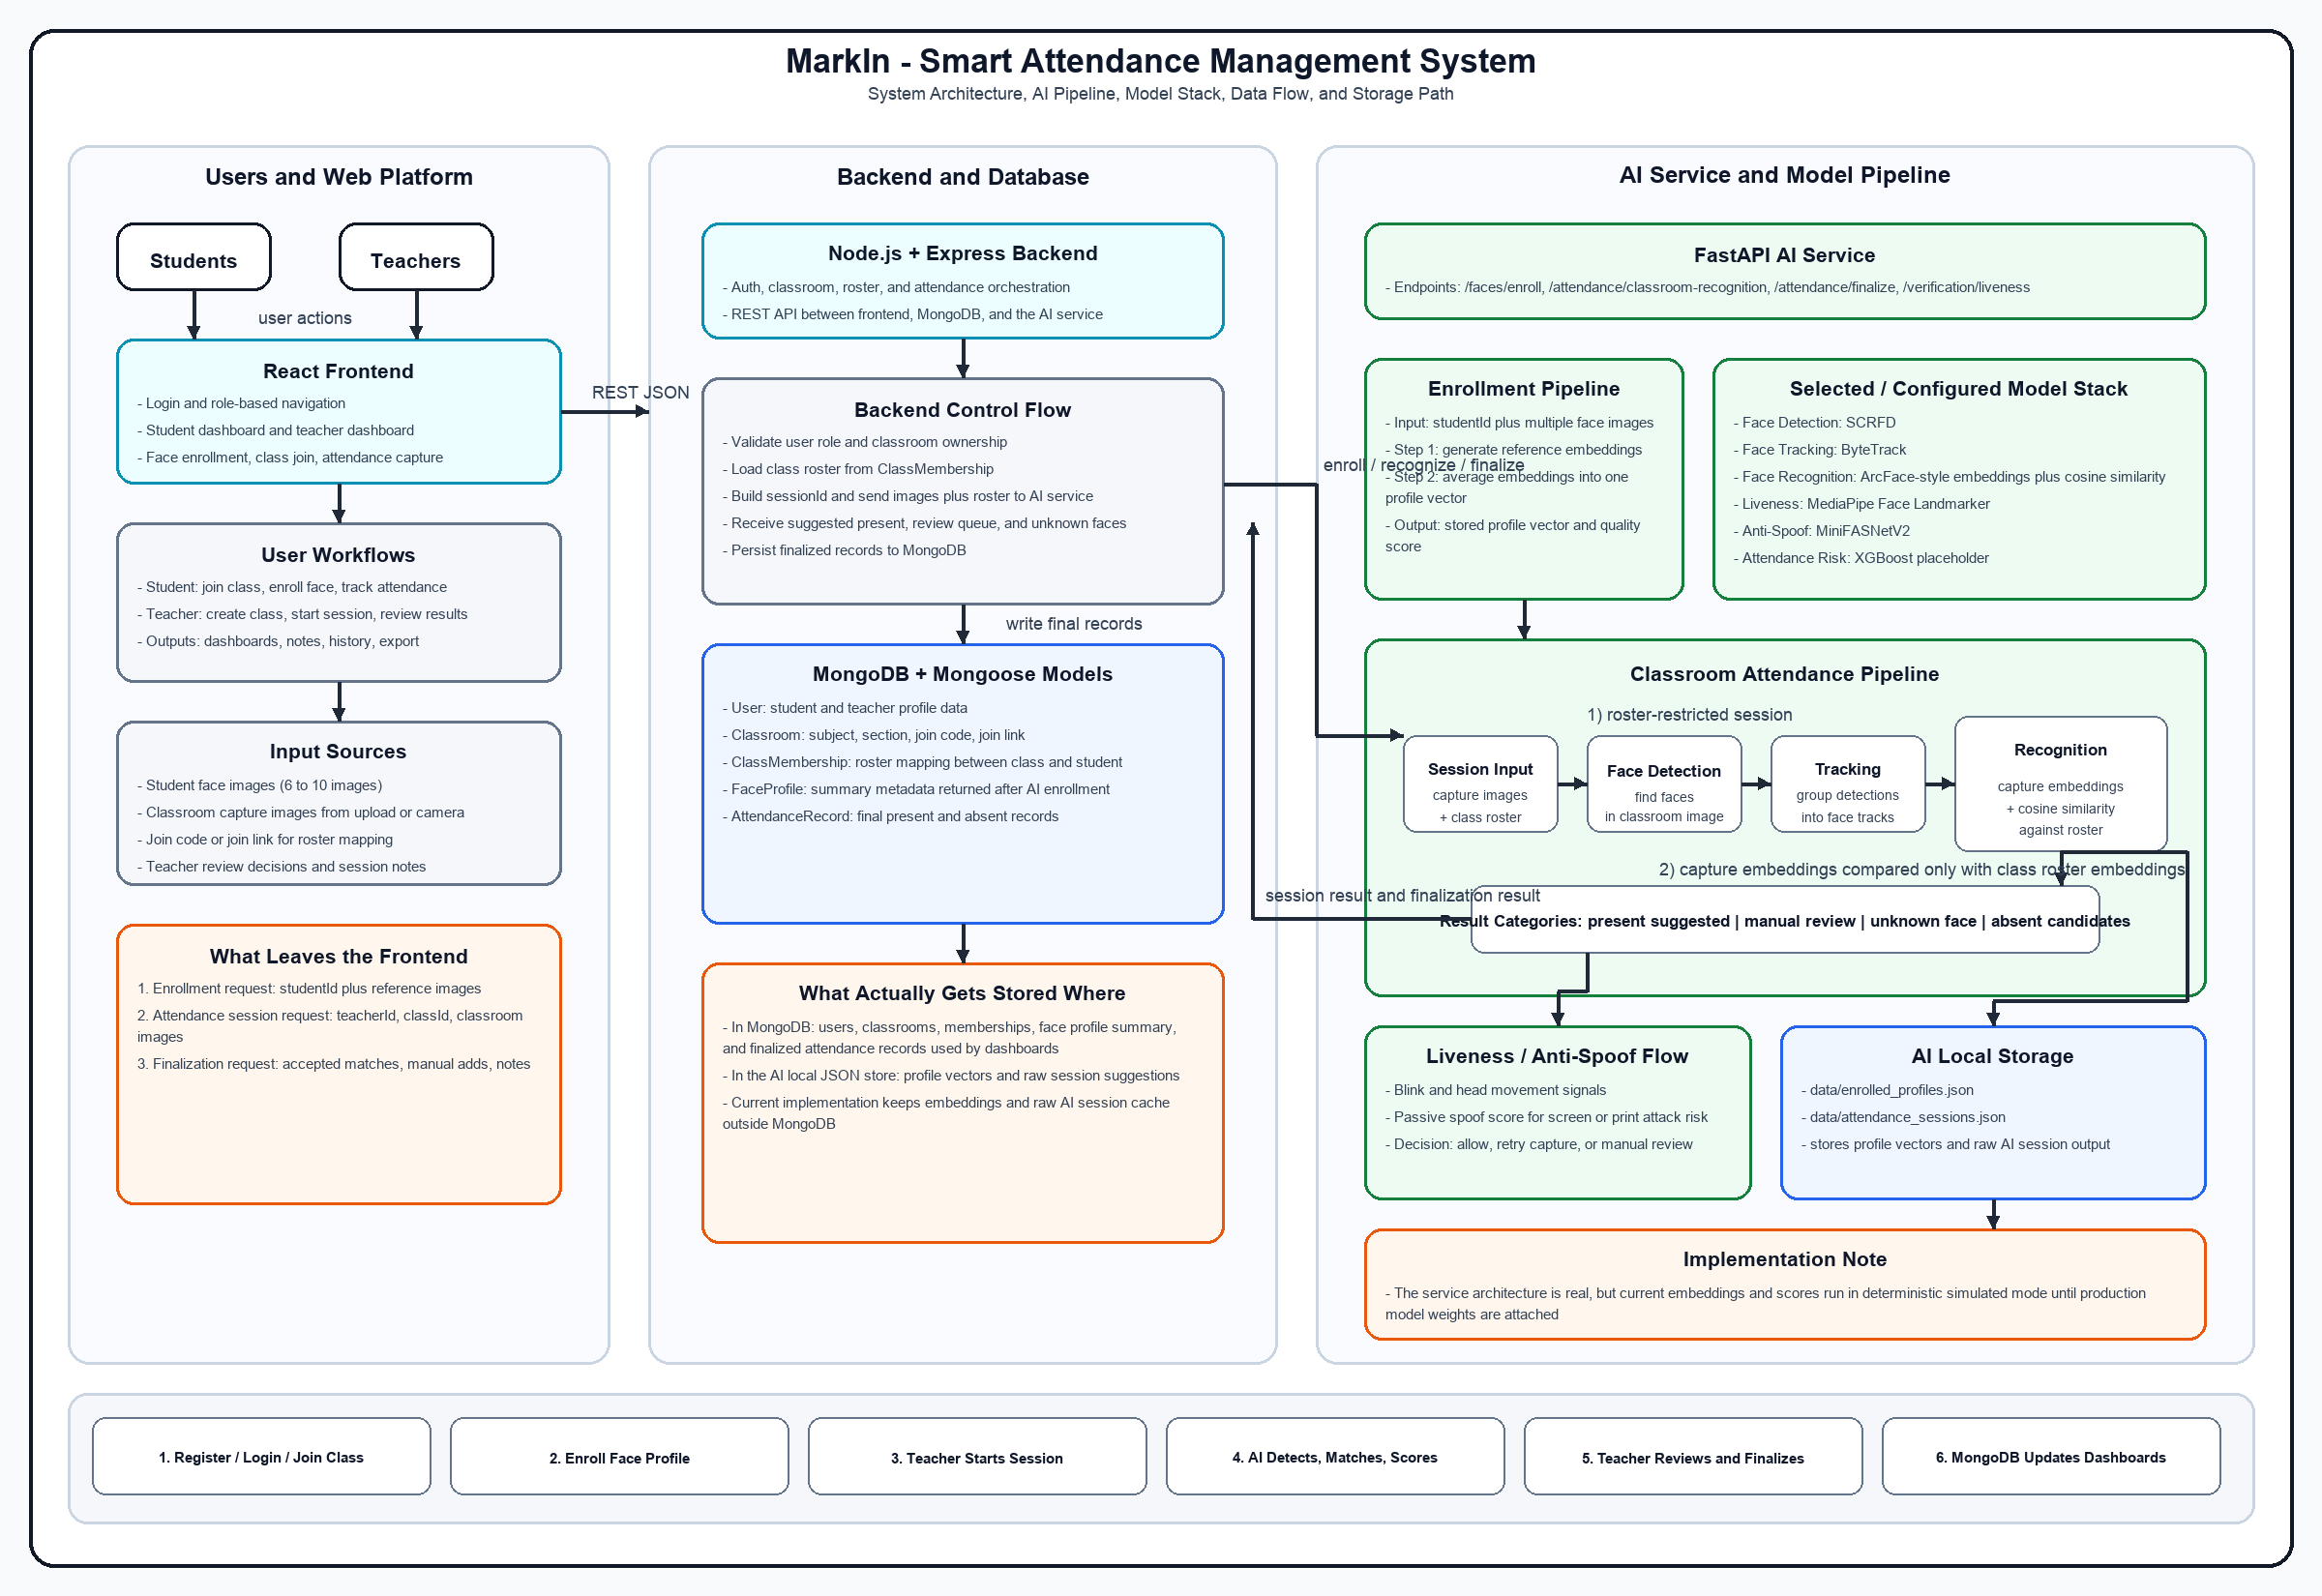
\includegraphics[width=0.96\textwidth]{markin-system-architecture-workflow.png}
\caption{Overall MarkIn/SAMS architecture and workflow}
\label{fig:repo-architecture}
\end{figure}

\begin{figure}[H]
\centering
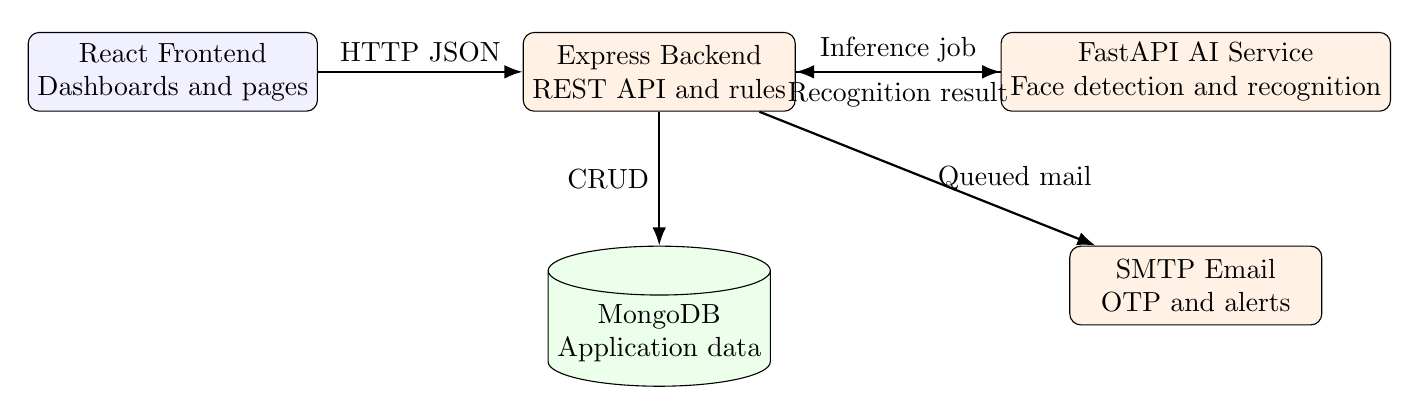
\begin{tikzpicture}[
box/.style={draw, rounded corners, align=center, minimum height=1cm, minimum width=3.1cm, fill=blue!6},
store/.style={draw, cylinder, shape border rotate=90, aspect=0.22, align=center, minimum height=1.2cm, minimum width=2.5cm, fill=green!8},
svc/.style={draw, rounded corners, align=center, minimum height=1cm, minimum width=3.2cm, fill=orange!10},
arrow/.style={-Latex, thick}
]
\node[box] (ui) {React Frontend\\Dashboards and pages};
\node[svc, right=2.6cm of ui] (api) {Express Backend\\REST API and rules};
\node[svc, right=2.6cm of api] (ai) {FastAPI AI Service\\Face detection and recognition};
\node[store, below=1.7cm of api] (db) {MongoDB\\Application data};
\node[svc, below=1.7cm of ai] (smtp) {SMTP Email\\OTP and alerts};
\draw[arrow] (ui) -- node[above]{HTTP JSON} (api);
\draw[arrow] (api) -- node[above]{Inference job} (ai);
\draw[arrow] (api) -- node[left]{CRUD} (db);
\draw[arrow] (api) -- node[right]{Queued mail} (smtp);
\draw[arrow] (ai) -- node[below]{Recognition result} (api);
\end{tikzpicture}
\caption{Service-level communication}
\label{fig:service-communication}
\end{figure}

\section{Frontend Design}

The frontend is built with React and JavaScript. It contains separate pages for the home page, authentication, student dashboard, student tools, student class detail, face enrollment, QR attendance, teacher dashboard, teacher class creation, teacher profile and teacher classroom students. The frontend service layer in \texttt{frontend/src/services/api.js} centralizes API calls so that pages do not duplicate endpoint strings and error handling.

The frontend design is role-oriented. After login, a student sees attendance health, classes joined, upcoming exams, notification count and tools such as the attendance calculator. The class detail page gives a separate view for each class, including attendance history, schedule and leave proof form. A teacher sees classes, schedule, student lists, attendance controls, Today Attendance Data and leave reviews.

\section{Backend Design}

The backend is built with Express and Mongoose. It exposes REST endpoints under the API router. Controllers receive requests and services contain reusable business logic. Models define MongoDB schemas. This separation allows the project to grow without placing all logic inside routes.

\begin{table}[H]
\centering
\caption{Backend layer responsibilities}
\label{tab:backend-layers}
\begin{tabularx}{\textwidth}{p{3.2cm} X X}
\toprule
\textbf{Layer} & \textbf{Examples} & \textbf{Responsibility}\\
\midrule
Routes & \texttt{backend/src/routes/index.js} & Maps URL paths and HTTP verbs to controllers.\\
Controllers & Auth, student, teacher, classroom and attendance controllers & Validate request shape, call services and return JSON responses.\\
Services & Email, attendance, dashboard, leave, exam and AI gateway services & Implement business rules, calculations and integrations.\\
Models & User, Classroom, AttendanceRecord, AttendanceDraft and others & Define persistent document structure and indexes.\\
Configuration & Environment and database configuration & Loads safe runtime settings and connects to MongoDB.\\
\bottomrule
\end{tabularx}
\end{table}

\section{AI Service Design}

The AI service is separated from the backend because face recognition has different dependencies and lifecycle needs. It is written with FastAPI and contains routes, services, pipelines, storage helpers and schemas. The relevant pipelines include enrollment, live verification and classroom attendance. The system can use InsightFace model packs such as Antelopev2 or Buffalo\_L, depending on available local assets.

In the attendance workflow, the backend sends classroom images and enrolled face profiles to the AI service. The AI service detects faces, extracts embeddings, compares them with enrolled student profiles and returns a result with matched students, unmatched faces and confidence notes. The teacher sees useful verification notes rather than every raw internal score.

\section{Database Design}

MongoDB stores the state of the system as collections. A simplified entity relationship view is shown in Figure~\ref{fig:er-diagram}. Although MongoDB is document-oriented, the application still has relationships through ids such as \texttt{classId}, \texttt{studentUserId} and \texttt{teacherUserId}.

\begin{figure}[H]
\centering
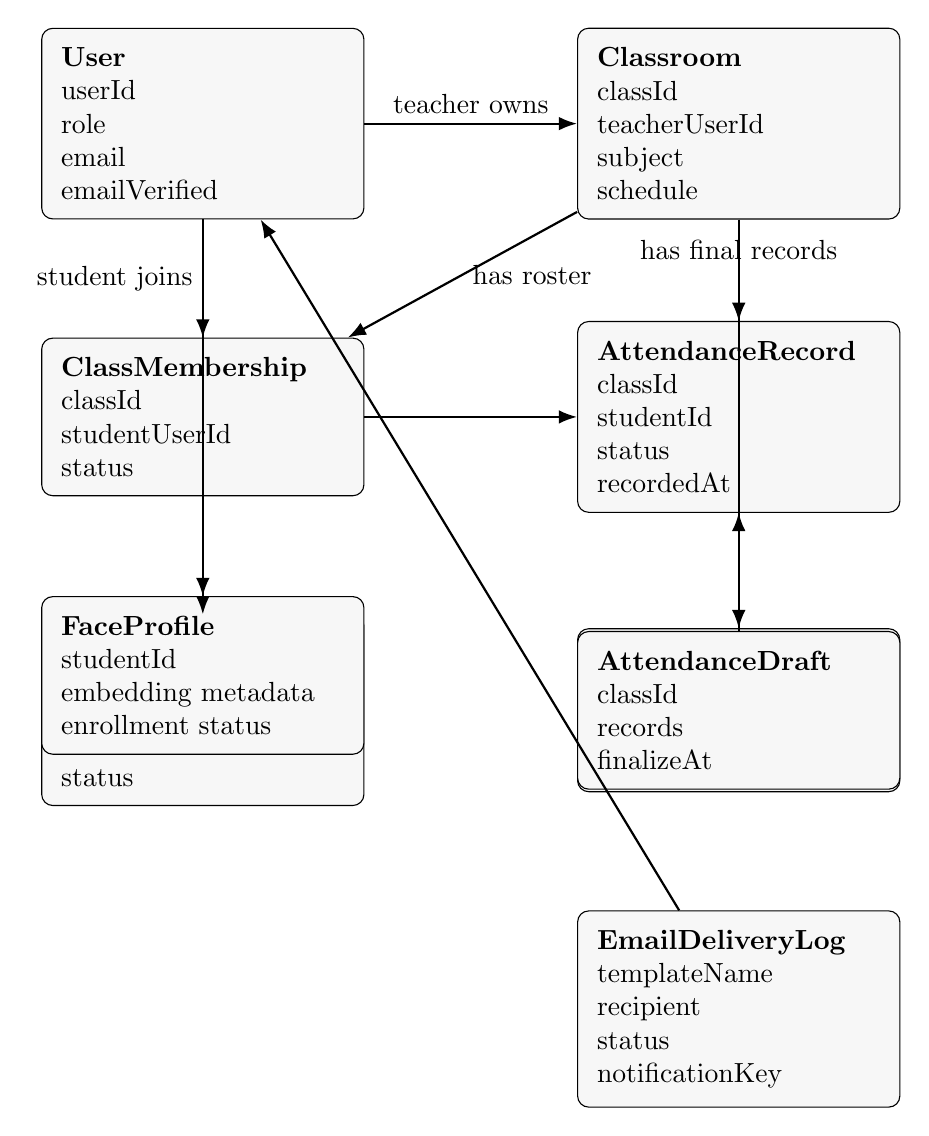
\begin{tikzpicture}[
entity/.style={draw, rounded corners, align=left, text width=3.6cm, fill=gray!6, inner sep=7pt},
rel/.style={-Latex, thick}
]
\node[entity] (user) {\textbf{User}\\userId\\role\\email\\emailVerified};
\node[entity, right=2.7cm of user] (class) {\textbf{Classroom}\\classId\\teacherUserId\\subject\\schedule};
\node[entity, below=1.5cm of user] (member) {\textbf{ClassMembership}\\classId\\studentUserId\\status};
\node[entity, right=2.7cm of member] (record) {\textbf{AttendanceRecord}\\classId\\studentId\\status\\recordedAt};
\node[entity, below=1.5cm of member] (leave) {\textbf{LeaveRequest}\\classId\\studentUserId\\attachments\\status};
\node[entity, right=2.7cm of leave] (exam) {\textbf{ClassExam}\\classId\\examDate\\requiredPercentage};
\node[entity, below=1.5cm of user] (face) at ($(user)+(0,-4.5)$) {\textbf{FaceProfile}\\studentId\\embedding metadata\\enrollment status};
\node[entity, below=1.5cm of record] (draft) {\textbf{AttendanceDraft}\\classId\\records\\finalizeAt};
\node[entity, below=1.5cm of exam] (mail) {\textbf{EmailDeliveryLog}\\templateName\\recipient\\status\\notificationKey};
\draw[rel] (user) -- node[above]{teacher owns} (class);
\draw[rel] (user) -- node[left]{student joins} (member);
\draw[rel] (class) -- node[right]{has roster} (member);
\draw[rel] (class) -- node[above]{has final records} (record);
\draw[rel] (member) -- (record);
\draw[rel] (member) -- (leave);
\draw[rel] (class) -- (exam);
\draw[rel] (user) -- (face);
\draw[rel] (draft) -- (record);
\draw[rel] (mail) -- (user);
\end{tikzpicture}
\caption{Simplified database/entity relationship diagram}
\label{fig:er-diagram}
\end{figure}

\begin{table}[H]
\centering
\caption{Database collection summary}
\label{tab:collection-summary}
\begin{tabularx}{\textwidth}{p{3.6cm} X}
\toprule
\textbf{Collection} & \textbf{Purpose}\\
\midrule
\texttt{users} & Stores student and teacher accounts, profile details and email verification state.\\
\texttt{classrooms} & Stores class identity, teacher ownership, schedule, room and join code.\\
\texttt{classmemberships} & Stores student membership in classes.\\
\texttt{attendancerecords} & Stores finalized attendance entries used for analytics.\\
\texttt{attendancedrafts} & Stores Today Attendance Data before final submission.\\
\texttt{faceprofiles} & Stores face enrollment metadata for student recognition.\\
\texttt{leaverequests} & Stores medical or leave proof, attachments and teacher review state.\\
\texttt{classexams} & Stores exam dates and required attendance percentages.\\
\texttt{emailotps} & Stores temporary OTP entries with expiry and purpose.\\
\texttt{emaildeliverylogs} & Stores email delivery attempts, status and errors.\\
\texttt{qrattendancesessions} & Stores QR session windows and class attendance scan state.\\
\texttt{classassignments} & Stores assignments created by teachers.\\
\texttt{classassignmentsubmissions} & Stores student assignment submissions.\\
\texttt{classdiscussionmessages} & Stores class discussion posts, replies and reactions.\\
\bottomrule
\end{tabularx}
\end{table}

\section{Today Attendance Data Design}

The Today Attendance Data feature is one of the most important project workflows. The design avoids a common weakness of automatic attendance systems: immediately writing AI output as final attendance. Instead, the backend creates a draft. The draft has a list of present and absent students, recognition notes, source photos, timestamps and finalization status. The draft remains editable for the teacher. The system can send absence notifications as soon as the draft is created, but final records are written only when the teacher finalizes or the automatic finalization period expires.

\begin{figure}[H]
\centering
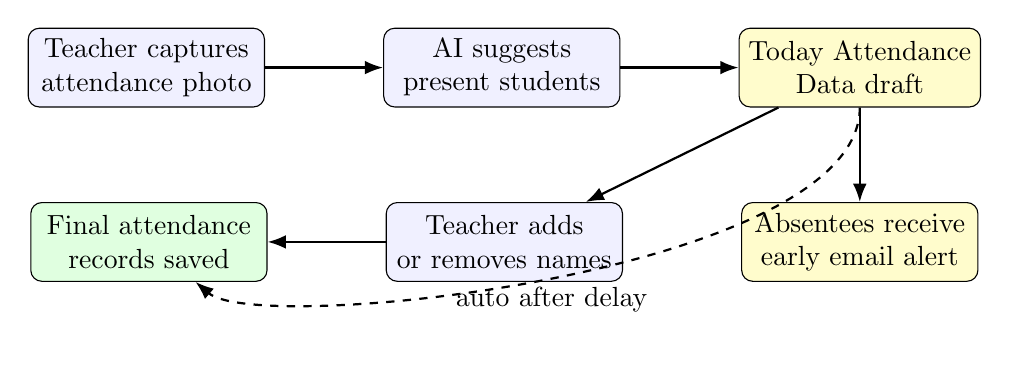
\begin{tikzpicture}[
flowstep/.style={draw, rounded corners, align=center, minimum width=3cm, minimum height=1cm, fill=blue!6},
warn/.style={draw, rounded corners, align=center, minimum width=3cm, minimum height=1cm, fill=yellow!20},
done/.style={draw, rounded corners, align=center, minimum width=3cm, minimum height=1cm, fill=green!12},
arrow/.style={-Latex, thick}
]
\node[flowstep] (photo) {Teacher captures\\attendance photo};
\node[flowstep, right=1.5cm of photo] (ai) {AI suggests\\present students};
\node[warn, right=1.5cm of ai] (draft) {Today Attendance\\Data draft};
\node[warn, below=1.2cm of draft] (email) {Absentees receive\\early email alert};
\node[flowstep, left=1.5cm of email] (review) {Teacher adds\\or removes names};
\node[done, left=1.5cm of review] (final) {Final attendance\\records saved};
\draw[arrow] (photo) -- (ai);
\draw[arrow] (ai) -- (draft);
\draw[arrow] (draft) -- (email);
\draw[arrow] (draft) -- (review);
\draw[arrow] (review) -- (final);
\draw[arrow, dashed] (draft) .. controls +(0,-2.6) and +(1.4,-1.2) .. node[below]{auto after delay} (final);
\end{tikzpicture}
\caption{Today Attendance Data draft and finalization flow}
\label{fig:today-attendance-flow}
\end{figure}

\section{Email Notification Architecture}

Email is handled by a dedicated backend module using Nodemailer. The service is configurable through environment variables. Email sending is disabled by default in development unless explicitly enabled. When enabled, the service verifies SMTP connectivity, uses professional templates and records delivery status. The email module does not print credentials in status responses.

\begin{figure}[H]
\centering
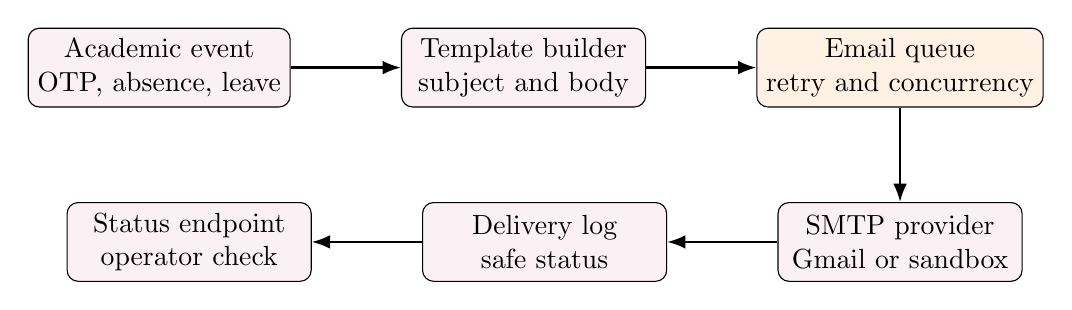
\begin{tikzpicture}[
box/.style={draw, rounded corners, align=center, minimum width=3.1cm, minimum height=1cm, fill=purple!6},
queue/.style={draw, rounded corners, align=center, minimum width=3.1cm, minimum height=1cm, fill=orange!10},
arrow/.style={-Latex, thick}
]
\node[box] (event) {Academic event\\OTP, absence, leave};
\node[box, right=1.4cm of event] (template) {Template builder\\subject and body};
\node[queue, right=1.4cm of template] (queue) {Email queue\\retry and concurrency};
\node[box, below=1.2cm of queue] (smtp) {SMTP provider\\Gmail or sandbox};
\node[box, left=1.4cm of smtp] (log) {Delivery log\\safe status};
\node[box, left=1.4cm of log] (dashboard) {Status endpoint\\operator check};
\draw[arrow] (event) -- (template);
\draw[arrow] (template) -- (queue);
\draw[arrow] (queue) -- (smtp);
\draw[arrow] (smtp) -- (log);
\draw[arrow] (log) -- (dashboard);
\end{tikzpicture}
\caption{Email notification flow}
\label{fig:email-flow}
\end{figure}

\section{Security Design}

The most important security decisions are simple and practical. Credentials stay in backend environment variables. The frontend never receives SMTP password, database URL or AI model paths. The email status endpoint returns only safe information such as enabled state, host name, sender and verification status. OTP records have an expiry time. Profile email updates require OTP verification. Leave attachments are shown through controlled application data rather than requiring teachers to download files blindly.

For a production version, this design should be extended with stronger session management, role-based middleware, rate limits for OTP requests, file size restrictions, antivirus scanning for uploaded documents and more detailed audit logs. The current design already keeps the main sensitive values away from public pages and report content.

\section{API Design Style}

The REST API uses resource-oriented routes. For example, student dashboard data is requested using a student id, teacher class actions use teacher id and class id, and leave review uses request id. This makes URLs readable and helps map actions to the user role.

\begin{table}[H]
\centering
\caption{Representative API design examples}
\label{tab:api-design-examples}
\begin{tabularx}{\textwidth}{p{2.3cm} p{5.4cm} X}
\toprule
\textbf{Method} & \textbf{Path} & \textbf{Purpose}\\
\midrule
GET & \texttt{/api/v1/students/:userId/dashboard} & Load student analytics, classes, notifications and exam information.\\
POST & \texttt{/api/v1/students/:studentId/classes/join} & Join a class using a teacher-provided join code.\\
POST & \texttt{/api/v1/teachers/:teacherId/classes/:classId/attendance/session} & Process AI-assisted photo attendance and create a Today Attendance Data draft.\\
PATCH & \texttt{/api/v1/teachers/:teacherId/classes/:classId/attendance/today-draft/:draftId} & Edit a draft by adding or removing students before final submission.\\
POST & \texttt{/api/v1/teachers/:teacherId/classes/:classId/attendance/today-draft/:draftId/finalize} & Convert a draft into final attendance records.\\
PATCH & \texttt{/api/v1/teachers/:teacherId/classes/:classId/exam} & Set or update exam date and required attendance percentage.\\
\bottomrule
\end{tabularx}
\end{table}

This chapter explained how the system is arranged. The next chapter explains how these designs are implemented in code.

\chapter{Implementation Details}
\label{chap:implementation}

This chapter explains how the design is converted into working software. The project is implemented as a monorepo with three application services. The frontend handles browser pages, the backend handles API and business rules, and the AI service handles face recognition pipelines. The implementation is intentionally modular so that one part can be improved without rewriting the entire application.

\section{Project Structure}

The top-level project structure keeps related code together. A beginner reading the repository can first identify the service and then inspect the pages, controllers, services or models inside it.

\begin{verbatim}
SAMS/
  frontend/      React and Parcel user interface
  backend/       Express REST API, Mongoose models and services
  ai-service/    FastAPI face recognition service
  docs/          Architecture, roadmap and email notes
  reports/       Generated LaTeX report workspace
  docker-compose.yml
\end{verbatim}

The backend also contains a service-oriented structure:

\begin{verbatim}
backend/src/
  controllers/   Request handlers for API routes
  models/        Mongoose schemas
  routes/        Central API router
  services/      Business logic and integrations
  config/        Environment and database setup
\end{verbatim}

\section{Technology Stack}

The chosen technologies are common enough for student developers to understand and powerful enough to support the required features. Table~\ref{tab:tech-stack-implementation} summarizes the stack.

\begin{table}[H]
\centering
\caption{Technology stack used in implementation}
\label{tab:tech-stack-implementation}
\begin{tabularx}{\textwidth}{p{3.2cm} p{4cm} X}
\toprule
\textbf{Layer} & \textbf{Technology} & \textbf{Reason for use}\\
\midrule
Frontend & React, JavaScript, Parcel & Component-based UI with fast local development and reusable dashboard sections.\\
Backend & Node.js, Express & Simple REST API framework suitable for authentication, dashboards and attendance workflows.\\
Database & MongoDB, Mongoose & Flexible document storage with schemas for users, classes, records, leave requests and drafts.\\
AI service & Python, FastAPI & Clean API layer for face recognition pipelines and model readiness endpoints.\\
Face recognition & InsightFace model packs & Provides practical face detection and embedding-based recognition capability.\\
Email & Nodemailer, SMTP & Supports Gmail app passwords or free SMTP sandbox services.\\
Development & npm workspaces, Docker & Allows local multi-service development and container-based deployment.\\
Documentation & LaTeX & Produces a formal, editable and printable academic report.\\
\bottomrule
\end{tabularx}
\end{table}

\section{Backend Implementation}

The backend starts with configuration, database connection and route registration. API routes are grouped inside \texttt{backend/src/routes/index.js}. This single router maps paths to controllers. Controllers then call services. For example, authentication routes call authentication and OTP services, while teacher classroom routes call attendance, classroom, leave and exam services.

The service layer is the most important backend implementation decision. It prevents controllers from becoming too large. For example, \texttt{studentDashboardService.js} prepares student dashboard data, \texttt{attendanceAnalyticsService.js} summarizes records, \texttt{emailNotificationService.js} chooses notification templates, and \texttt{attendanceDraftScheduler.js} handles automatic draft finalization.

\subsection{Authentication and Email Verification}

During signup, the backend creates the user in a verification-required state and sends an OTP email. The user becomes active only after the OTP is verified. This prevents invalid or mistyped email addresses from receiving future academic alerts. Password reset also uses a secure temporary OTP flow. Profile email update uses a separate OTP purpose so that changing an email address cannot happen silently.

\begin{figure}[H]
\centering
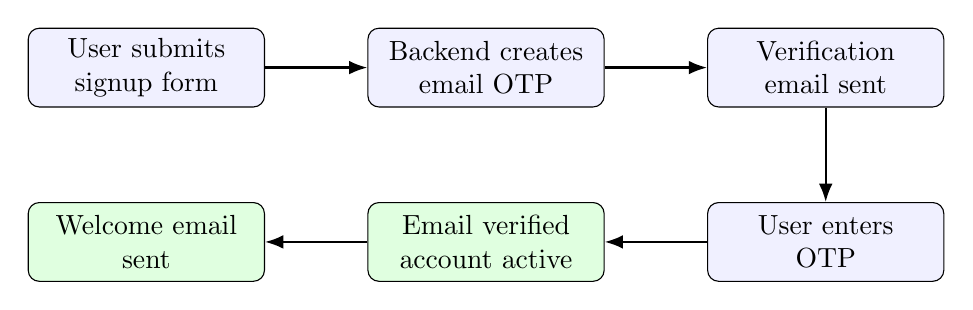
\begin{tikzpicture}[
flowstep/.style={draw, rounded corners, align=center, minimum width=3cm, minimum height=1cm, fill=blue!6},
ok/.style={draw, rounded corners, align=center, minimum width=3cm, minimum height=1cm, fill=green!12},
arrow/.style={-Latex, thick}
]
\node[flowstep] (signup) {User submits\\signup form};
\node[flowstep, right=1.3cm of signup] (otp) {Backend creates\\email OTP};
\node[flowstep, right=1.3cm of otp] (mail) {Verification\\email sent};
\node[flowstep, below=1.2cm of mail] (verify) {User enters\\OTP};
\node[ok, left=1.3cm of verify] (active) {Email verified\\account active};
\node[ok, left=1.3cm of active] (welcome) {Welcome email\\sent};
\draw[arrow] (signup) -- (otp);
\draw[arrow] (otp) -- (mail);
\draw[arrow] (mail) -- (verify);
\draw[arrow] (verify) -- (active);
\draw[arrow] (active) -- (welcome);
\end{tikzpicture}
\caption{Email verified registration implementation flow}
\label{fig:registration-flow}
\end{figure}

\subsection{Classroom and Membership Implementation}

The classroom module stores the teacher id, class details, schedule slots and join code. A class schedule slot includes weekday and time information. When a student joins a class, the backend creates a membership document. Attendance analytics later use the membership list to know which students belong to a class and which students must appear in class-level calculations.

The join-code design is simple and practical. A teacher can share a code or link. A student can join without the teacher manually typing every name. At the same time, the teacher can still add, update or remove students from the roster page, which is important when data is incomplete.

\subsection{Attendance Implementation}

The attendance implementation supports several sources. Manual attendance is direct. QR attendance uses a teacher-created session and a student scan endpoint. AI photo attendance sends image data to the AI service and produces a draft. All final records are stored in the attendance record collection with status and source fields.

\begin{table}[H]
\centering
\caption{Attendance status and meaning}
\label{tab:attendance-status}
\begin{tabularx}{\textwidth}{p{3cm} X X}
\toprule
\textbf{Status} & \textbf{Meaning} & \textbf{Typical source}\\
\midrule
Present & Student attended the class. & Manual, QR or AI-assisted session.\\
Absent & Student did not attend or was not confirmed present. & Draft finalization or manual entry.\\
Late & Student attended after expected time. & Manual teacher decision.\\
Excused & Student's absence is accepted through proof or teacher decision. & Leave review or manual decision.\\
Class cancelled & Class did not happen and should not harm attendance. & Teacher cancellation workflow.\\
\bottomrule
\end{tabularx}
\end{table}

\subsection{Today Attendance Draft Implementation}

When AI-assisted attendance is run, the backend does not immediately create final attendance records. It creates an \texttt{AttendanceDraft}. The draft includes class id, teacher id, recognized records, suggested present list, suggested absent list, verification notes and a finalization time. The teacher can update this draft using the draft update endpoint. Finalization converts the draft to attendance records.

This design supports a useful human-in-the-loop workflow. Suppose a student was present but hidden behind another student in the photo. The AI result might mark that student absent. The absent email gives the student a chance to tell the teacher. The teacher can then add the student in Today Attendance Data before final submission. This keeps the system useful without pretending that computer vision is perfect.

\section{Student Dashboard Implementation}

The student dashboard is implemented as a summary page supported by separate pages for tools and class details. The dashboard service computes totals, percentages, attendance trend, joined classes, upcoming exams and warnings. The frontend uses that data to show helpful cards and links.

\begin{table}[H]
\centering
\caption{Student dashboard data shown to users}
\label{tab:student-dashboard-data}
\begin{tabularx}{\textwidth}{p{3.5cm} X}
\toprule
\textbf{Data item} & \textbf{Student value}\\
\midrule
Classes joined & Shows how many active academic classes the student belongs to.\\
Total sessions held & Shows total attendance opportunities already recorded.\\
Present and absent counts & Converts percentage into understandable numbers.\\
Attendance percentage & Helps student know current standing.\\
Class-wise cards & Allows student to open a separate detail page for every class.\\
Upcoming exams & Connects attendance percentage to exam eligibility.\\
Minimum classes to attend & Shows a clear action target rather than only a warning.\\
Notification count & Alerts the student about risky classes, exams and leave decisions.\\
Face enrollment status & Reminds student to complete enrollment for photo attendance.\\
\bottomrule
\end{tabularx}
\end{table}

\section{Teacher Dashboard Implementation}

The teacher dashboard focuses on action. A teacher can create classes, see schedule, open class management, run attendance, create assignments, set exam rules and review leave requests. The teacher class students page provides roster analytics, low-attendance filters and a detailed student section. This is where teachers can preview leave proof files such as PDF or images online and approve or reject them.

Teacher actions are scoped by teacher id and class id. This makes it possible for the backend to verify that a teacher is operating on their own class before changing attendance, roster or exam data.

\section{Leave and Medical Proof Implementation}

The leave request feature is implemented in the student class detail page and teacher classroom students page. A student selects a request type, absence date, reason and attachment files. Files are converted to safe attachment metadata that the backend stores with the request. The teacher can open the student detail section and preview attachments. Images are shown inline and PDFs are shown in a browser preview area. The teacher can approve or reject with an optional note.

When the decision is saved, the email notification module sends a leave review email. The email contains the class, absence date and approval status. This helps students know the decision without repeatedly checking the dashboard.

\section{Exam Schedule and Eligibility Implementation}

The teacher can set an exam date and required attendance percentage for a class. The backend stores this in the class exam model. The student dashboard reads upcoming exams and calculates eligibility using current attendance and scheduled classes before the exam. The calculation can explain whether the student is currently safe, close to risk or below requirement.

The attendance calculator allows the student to enter an exam date and required percentage. The system can use the class schedule to estimate how many classes may be held before that exam date. The output is the minimum number of classes the student should attend to be safe. The general formula is:

\[
\text{required presents} = \left\lceil \frac{p}{100} \times \text{projected total classes} \right\rceil
\]

\[
\text{minimum future attendance} = \max(0, \text{required presents} - \text{current presents})
\]

Here \(p\) is the required attendance percentage. If the minimum future attendance is greater than the number of classes expected before the exam, then the student cannot mathematically reach the required percentage by only attending future classes. The dashboard can then show a stronger warning.

\section{Email Service Implementation}

The email system is implemented as a modular notification layer. It contains template builders, a sending service, OTP service and notification service. The environment controls whether email is enabled, which SMTP host is used, how many retries are allowed and whether OTPs can be exposed during development. In real operation, OTPs are not returned in API responses.

\begin{longtable}{p{3.2cm} p{4.2cm} p{6cm}}
\caption{Email notification events implemented in the backend}
\label{tab:email-events-implementation}\\
\toprule
\textbf{Event} & \textbf{Trigger} & \textbf{Email content}\\
\midrule
\endfirsthead
\toprule
\textbf{Event} & \textbf{Trigger} & \textbf{Email content}\\
\midrule
\endhead
Signup verification & New student or teacher registration & OTP, expiry and verification instructions.\\
Welcome message & Successful email verification & Student or teacher name, login email and account activation confirmation.\\
Password reset & User requests recovery & OTP or secure reset instructions and expiry warning.\\
Profile email OTP & User updates profile email & OTP for confirming the new email address.\\
Leave decision & Teacher approves or rejects a request & Class, leave date, status and teacher note when available.\\
Exam warning & Attendance below exam criterion & Current percentage, required percentage and action needed.\\
Absent notice & Student marked absent in draft or record & Class, date, subject and timing context.\\
Class cancellation & Teacher cancels or reschedules & Updated class information and schedule note.\\
\bottomrule
\end{longtable}

\section{AI Attendance Implementation}

The AI service contains three main pipeline areas: enrollment, live verification and classroom attendance. During enrollment, the student's face profile is captured and stored. During classroom attendance, the service detects faces in the submitted image, creates embeddings and compares them with enrolled profiles. The output is a list of matched students and useful notes.

The backend treats the AI service as a dependency that may be healthy, ready or degraded. Health endpoints help show whether MongoDB and AI runtime are available. If the AI model pack is missing or the service is still starting, the app can show degraded state instead of silently failing.

\section{Frontend Navigation Implementation}

The frontend uses hash-based routing. This makes the app easy to run in local development without server-side route rewriting. Pages are organized around real user tasks:

\begin{itemize}
\item Student dashboard for overview.
\item Student class detail page for a single class.
\item Student tools pages for exams, notifications and calculator.
\item Teacher dashboard for class and schedule overview.
\item Teacher classroom students page for roster, attendance and leave review.
\item QR attendance page for scan-based attendance.
\item Face enrollment page for preparing AI attendance.
\end{itemize}

\section{Error Handling}

The backend returns clear error messages when required fields are missing or operations fail. Email delivery uses retry settings and delivery logs. The frontend shows user-facing failure text when dashboard loading, leave submission, attendance processing or email tests fail. The AI service exposes health and readiness endpoints so infrastructure issues can be separated from application logic errors.

\section{Configuration Management}

Configuration values are stored in environment files and should be different for development and production. The report intentionally does not include actual database URLs, SMTP passwords or model secrets. A safe configuration example is included in the appendix using placeholders. This is important because academic documentation is often shared, printed or uploaded, and it must not expose real credentials.

This chapter covered the implementation approach. The next chapter explains the working of the main features from the user's point of view.

\chapter{Features and Working}
\label{chap:features}

This chapter explains the working of the system as a user would experience it. The purpose is to make the project understandable even for a reader who has not opened the code. Every major feature is described as a workflow: what the user does, what the backend does and what result appears.

\section{Landing Page}

The landing page introduces the project as a smart attendance platform rather than a simple register. It explains the main workflows: AI photo attendance, Today Attendance Data, class-wise student dashboard, exam eligibility, leave proof review, email alerts and teacher controls. It is useful for a first-time viewer because it gives a quick idea of the product before login.

The landing page also performs a health check so developers can see whether the backend is reachable. In a real deployment this helps distinguish a frontend loading issue from a backend service issue.

\section{Registration and Login}

Registration starts by selecting the role and entering profile details. The system sends an email OTP. The user enters the OTP and the account becomes verified. After verification, the user can log in and access the role-specific dashboard.

\begin{figure}[H]
\centering
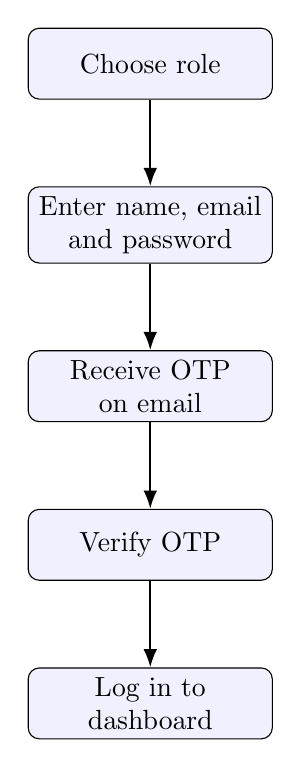
\begin{tikzpicture}[
node distance=1.1cm,
flowstep/.style={draw, rounded corners, align=center, minimum width=3.1cm, minimum height=0.9cm, fill=blue!6},
arrow/.style={-Latex, thick}
]
\node[flowstep] (role) {Choose role};
\node[flowstep, below=of role] (details) {Enter name, email\\and password};
\node[flowstep, below=of details] (otp) {Receive OTP\\on email};
\node[flowstep, below=of otp] (verify) {Verify OTP};
\node[flowstep, below=of verify] (login) {Log in to\\dashboard};
\draw[arrow] (role) -- (details);
\draw[arrow] (details) -- (otp);
\draw[arrow] (otp) -- (verify);
\draw[arrow] (verify) -- (login);
\end{tikzpicture}
\caption{Registration and login working}
\label{fig:registration-working}
\end{figure}

\section{Student Dashboard}

The student dashboard is designed to answer useful student questions quickly. It shows the number of classes joined, total classes held, present count, absent count, attendance percentage, risk state, upcoming exams and notification count. Each class card opens a separate class page so the dashboard does not become crowded.

\begin{table}[H]
\centering
\caption{Student dashboard feature matrix}
\label{tab:student-feature-matrix}
\begin{tabularx}{\textwidth}{p{3.7cm} X X}
\toprule
\textbf{Feature} & \textbf{What student sees} & \textbf{Why it is useful}\\
\midrule
Overview metrics & Joined classes, present, absent and percentage. & Converts attendance into simple academic status.\\
Class cards & Subject code, teacher, schedule and attendance health. & Lets student focus on one class at a time.\\
Notification bell & Count of exam, leave and attendance alerts. & Brings urgent items to attention.\\
Upcoming exams & Exam date, required percentage and eligibility. & Connects attendance to exam appearance risk.\\
Attendance calculator & Minimum future classes to attend. & Gives a clear plan instead of only a warning.\\
Face enrollment reminder & Profile readiness for AI attendance. & Reduces future recognition failures.\\
Leave request status & Pending, approved or rejected proof. & Avoids uncertainty after document upload.\\
\bottomrule
\end{tabularx}
\end{table}

\begin{figure}[H]
\centering
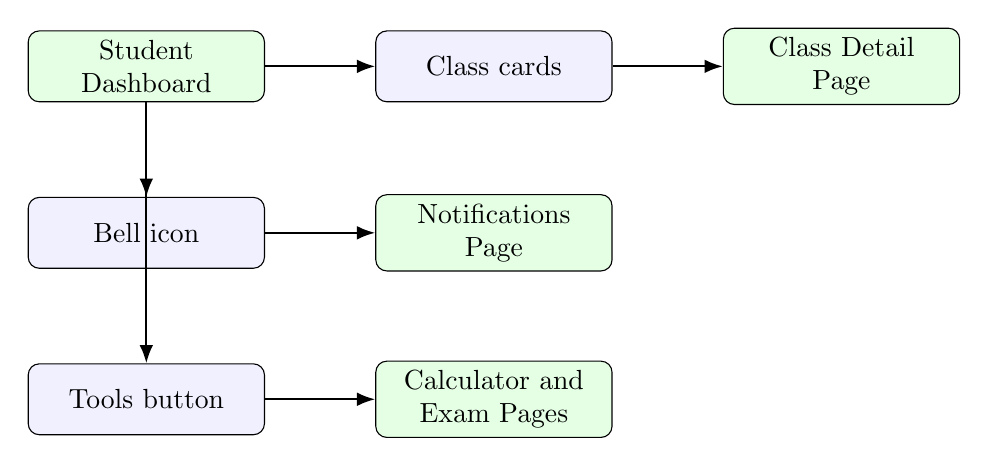
\begin{tikzpicture}[
box/.style={draw, rounded corners, align=center, minimum width=3cm, minimum height=0.9cm, fill=blue!6},
page/.style={draw, rounded corners, align=center, minimum width=3cm, minimum height=0.9cm, fill=green!10},
arrow/.style={-Latex, thick}
]
\node[page] (dash) {Student\\Dashboard};
\node[box, right=1.4cm of dash] (classcards) {Class cards};
\node[page, right=1.4cm of classcards] (classpage) {Class Detail\\Page};
\node[box, below=1.2cm of dash] (bell) {Bell icon};
\node[page, right=1.4cm of bell] (notify) {Notifications\\Page};
\node[box, below=1.2cm of bell] (tools) {Tools button};
\node[page, right=1.4cm of tools] (calc) {Calculator and\\Exam Pages};
\draw[arrow] (dash) -- (classcards);
\draw[arrow] (classcards) -- (classpage);
\draw[arrow] (dash) -- (bell);
\draw[arrow] (bell) -- (notify);
\draw[arrow] (dash) -- (tools);
\draw[arrow] (tools) -- (calc);
\end{tikzpicture}
\caption{Student dashboard navigation flow}
\label{fig:student-dashboard-flow}
\end{figure}

\section{Student Class Detail Page}

The class detail page is a focused page for one class. It shows attendance percentage, total sessions, missed sessions, recent records, regular schedule and class information. It also includes the leave proof form. The student can upload images or PDF files for medical reports, leave letters or absence reasons. The student can later see whether the request is pending, approved or rejected.

This separate page design is important. A student with many subjects should not have to read every detail on the main dashboard. The main dashboard gives summary and the class page gives depth.

\section{Attendance Calculator}

The attendance calculator is a planning tool. It takes current attendance percentage, current present and total counts, exam date, required eligibility percentage and expected number of future classes. When possible, future classes are estimated from the class schedule. The calculator then tells the student how many classes must be attended to reach the requirement safely.

\begin{table}[H]
\centering
\caption{Attendance calculator inputs and outputs}
\label{tab:calculator}
\begin{tabularx}{\textwidth}{p{3.4cm} X}
\toprule
\textbf{Input or output} & \textbf{Meaning}\\
\midrule
Current present count & Number of classes already attended.\\
Current total count & Number of classes already recorded.\\
Current percentage & Existing attendance standing.\\
Exam date & Date until which future classes are estimated.\\
Required percentage & Eligibility threshold set by teacher or entered by student.\\
Future classes & Number of scheduled classes before the exam.\\
Minimum required attendance & Number of future classes the student should attend.\\
Safety message & Explains whether the target is possible, safe or risky.\\
\bottomrule
\end{tabularx}
\end{table}

\section{Teacher Dashboard}

The teacher dashboard is designed for repeated classroom work. It provides class creation, class list, schedule, exam setup and access to each class. A teacher can create a subject with code, section, semester and schedule. The generated join code allows students to join. The teacher can open a class to see students, attendance performance, leave requests and attendance controls.

\section{Teacher Attendance Workflow}

The teacher has multiple ways to take attendance. Manual attendance is useful for small classes or corrections. QR attendance is useful for quick self-marking during a time-limited session. AI photo attendance is useful when the teacher wants to capture classroom presence quickly from images.

\begin{figure}[H]
\centering
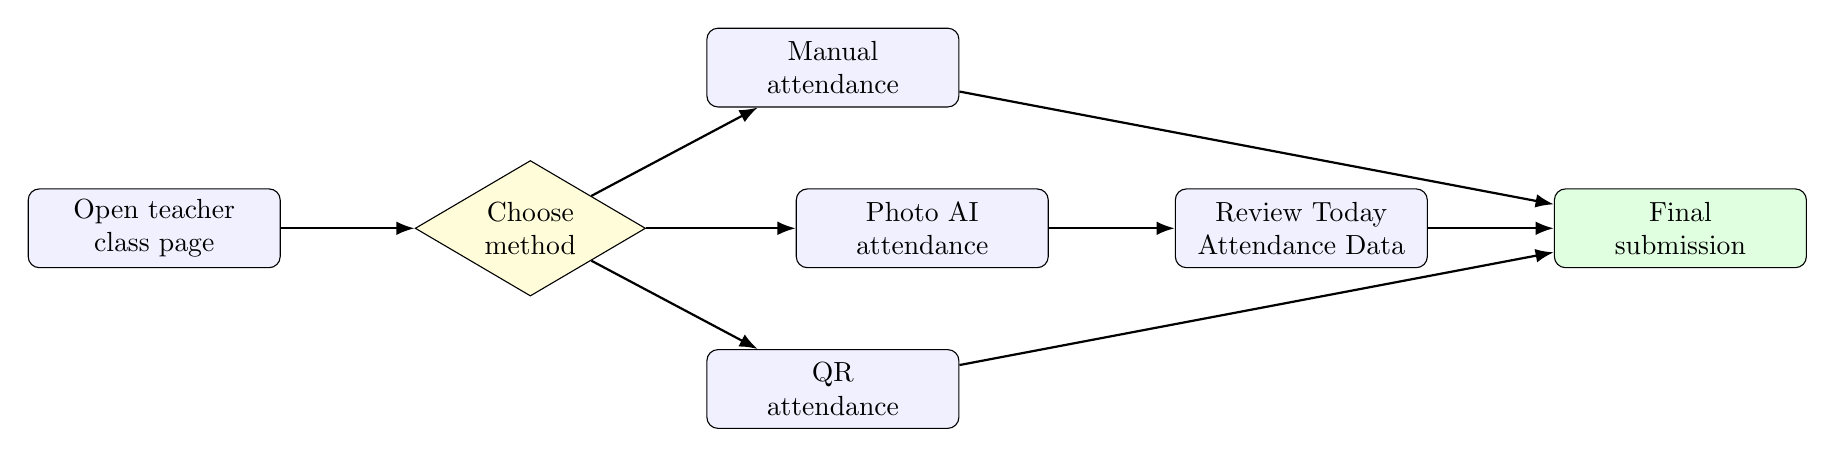
\begin{tikzpicture}[
flowstep/.style={draw, rounded corners, align=center, minimum width=3.2cm, minimum height=1cm, fill=blue!6},
choice/.style={draw, diamond, aspect=1.7, align=center, fill=yellow!15},
done/.style={draw, rounded corners, align=center, minimum width=3.2cm, minimum height=1cm, fill=green!12},
arrow/.style={-Latex, thick}
]
\node[flowstep] (open) {Open teacher\\class page};
\node[choice, right=1.7cm of open] (method) {Choose\\method};
\node[flowstep, above right=1.1cm and 1.5cm of method] (manual) {Manual\\attendance};
\node[flowstep, right=1.9cm of method] (photo) {Photo AI\\attendance};
\node[flowstep, below right=1.1cm and 1.5cm of method] (qr) {QR\\attendance};
\node[flowstep, right=1.6cm of photo] (draft) {Review Today\\Attendance Data};
\node[done, right=1.6cm of draft] (final) {Final\\submission};
\draw[arrow] (open) -- (method);
\draw[arrow] (method) -- (manual);
\draw[arrow] (method) -- (photo);
\draw[arrow] (method) -- (qr);
\draw[arrow] (manual) -- (final);
\draw[arrow] (qr) -- (final);
\draw[arrow] (photo) -- (draft);
\draw[arrow] (draft) -- (final);
\end{tikzpicture}
\caption{Teacher attendance workflow}
\label{fig:teacher-attendance-flow}
\end{figure}

\section{AI Photo Attendance}

In AI photo attendance, the teacher captures or uploads a classroom photo. The backend sends the photo to the AI service. The AI service detects faces and compares them with enrolled student face profiles. It returns matched students and verification notes. The teacher sees the result in a useful form: who is probably present, who is absent and which notes require attention.

The result goes to Today Attendance Data, not directly to final records. This is the key safety feature. Students who are marked absent receive an email early. If there is an error, the student can contact the teacher, and the teacher can correct the draft. This approach improves trust because the system is transparent and correctable.

\section{Today Attendance Data Section}

The Today Attendance Data section contains the current draft attendance for the day. It shows present students and absent students. The teacher can add a student to the present list, remove a student, change status and finalize. The draft can also be finalized automatically after the configured period, such as twelve hours, so that attendance does not remain pending forever.

\begin{table}[H]
\centering
\caption{Today Attendance Data actions}
\label{tab:today-actions}
\begin{tabularx}{\textwidth}{p{3.3cm} X X}
\toprule
\textbf{Action} & \textbf{Who performs it} & \textbf{Result}\\
\midrule
Create draft & Teacher through photo attendance workflow & AI suggested attendance is stored for review.\\
Notify absentees & Backend email module & Students marked absent receive early email warning.\\
Add student & Teacher & Corrects false absent or missed recognition.\\
Remove student & Teacher & Corrects false present or accidental entry.\\
Finalize manually & Teacher & Draft becomes final attendance records.\\
Finalize automatically & Scheduler & Draft is submitted after the configured waiting period.\\
\bottomrule
\end{tabularx}
\end{table}

\section{Leave Proof and Medical Report Workflow}

The leave proof workflow solves a common issue: students often have a valid reason for absence but proof is shared informally through messages. In SAMS, proof is connected to the class and date. The student submits the request from the class detail page. The teacher previews the document in the student detail section and approves or rejects it. The student receives an email and dashboard status update.

\begin{figure}[H]
\centering
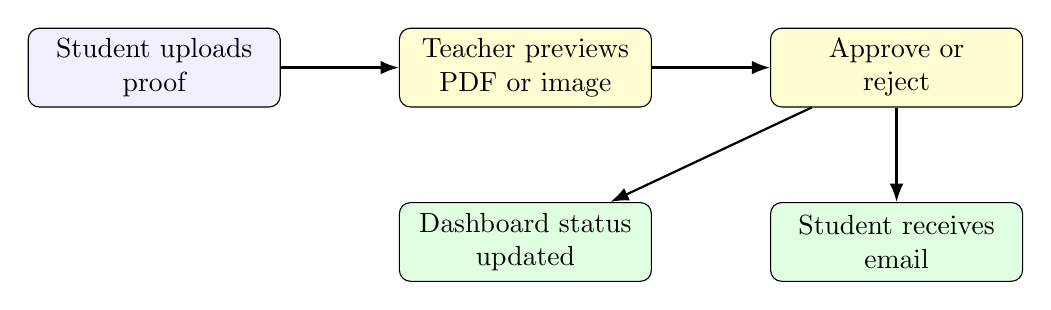
\begin{tikzpicture}[
flowstep/.style={draw, rounded corners, align=center, minimum width=3.2cm, minimum height=1cm, fill=blue!6},
review/.style={draw, rounded corners, align=center, minimum width=3.2cm, minimum height=1cm, fill=yellow!18},
done/.style={draw, rounded corners, align=center, minimum width=3.2cm, minimum height=1cm, fill=green!12},
arrow/.style={-Latex, thick}
]
\node[flowstep] (student) {Student uploads\\proof};
\node[review, right=1.5cm of student] (teacher) {Teacher previews\\PDF or image};
\node[review, right=1.5cm of teacher] (decision) {Approve or\\reject};
\node[done, below=1.2cm of decision] (email) {Student receives\\email};
\node[done, left=1.5cm of email] (status) {Dashboard status\\updated};
\draw[arrow] (student) -- (teacher);
\draw[arrow] (teacher) -- (decision);
\draw[arrow] (decision) -- (email);
\draw[arrow] (decision) -- (status);
\end{tikzpicture}
\caption{Leave proof review workflow}
\label{fig:leave-flow}
\end{figure}

\section{Exam Scheduling and Eligibility}

The teacher can define an upcoming exam for a class. The exam entry contains exam date, required attendance percentage and optional notes. The student dashboard uses current attendance and schedule information to show eligibility. If the student is below the required percentage, the dashboard and email warnings explain the problem.

This feature is more useful than a normal attendance percentage because it connects present behaviour to future consequence. A student can see how many classes must be attended before the exam. A teacher can warn students early instead of announcing ineligibility at the last moment.

\section{Notification Bell and Separate Pages}

The student dashboard includes a notification bell icon. It summarizes urgent items such as low attendance, upcoming exam risk, face enrollment reminder and leave request decision. The bell opens a separate notification page instead of expanding large content inside the dashboard. Similarly, tools such as the calculator and exams open on separate pages. This keeps the dashboard efficient and prevents it from becoming overloaded.

\section{Class Cancellation and Reschedule Notice}

If a class is cancelled or rescheduled, the teacher can update the class state. Students receive a bulk email notice with updated information. The attendance record can use a class-cancelled status so that cancelled sessions do not reduce student attendance percentage.

\section{Assignments and Class Discussion}

The project also includes class assignment and discussion features. Teachers can create assignments for a class, students can submit responses and class discussion messages can include replies or reactions. These features are useful because attendance systems are often part of a wider class management workflow. Keeping assignments and discussions in the same class context gives students one place to check academic activity.

\section{Feature Summary}

\begin{longtable}{p{3.5cm} p{4.8cm} p{5.1cm}}
\caption{Complete feature matrix}
\label{tab:complete-feature-matrix}\\
\toprule
\textbf{Feature} & \textbf{Student benefit} & \textbf{Teacher benefit}\\
\midrule
\endfirsthead
\toprule
\textbf{Feature} & \textbf{Student benefit} & \textbf{Teacher benefit}\\
\midrule
\endhead
Email verification & Ensures account email can receive alerts. & Ensures teacher account can send and receive system notices.\\
Class join code & Easy class joining. & Less manual roster creation.\\
Class-wise dashboard & Understands subject-specific performance. & Reduces repeated student queries.\\
Photo attendance & Less roll-call time. & Faster attendance with review controls.\\
QR attendance & Fast self-marking when allowed. & Useful alternative to photo recognition.\\
Today Attendance Data & Early chance to report mistakes. & Correctable draft before final submission.\\
Leave proof upload & Formal way to submit medical or leave documents. & Online review without downloading every file.\\
Exam eligibility & Clear target before exam. & Early warning for at-risk students.\\
Attendance calculator & Personal planning tool. & Reduces confusion about required classes.\\
Notification bell & Urgent items in one place. & Students see warnings without teacher repeating them.\\
Email alerts & Important changes reach inbox. & Automated communication for repetitive events.\\
Cancellation notice & Knows class changes quickly. & Bulk class communication.\\
\bottomrule
\end{longtable}

This chapter described the working features. The next chapter verifies these features through testing and result analysis.

\chapter{Testing and Results}
\label{chap:testing}

Testing verifies that the system works as expected and that important academic workflows do not silently fail. For SAMS, testing is especially important because attendance data affects students directly. The project therefore uses a combination of unit tests, service checks, manual workflow tests and document-level validation.

\section{Testing Strategy}

The testing strategy is based on risk. Features that can affect attendance records, email delivery or eligibility warnings require more careful checking. UI-only improvements can be checked through browser interaction and visual review. AI recognition pipelines need separate tests because they depend on model readiness, image input and stored face profiles.

\begin{table}[H]
\centering
\caption{Testing levels used for the project}
\label{tab:testing-levels}
\begin{tabularx}{\textwidth}{p{3cm} X X}
\toprule
\textbf{Level} & \textbf{Purpose} & \textbf{Examples}\\
\midrule
Unit testing & Verify a small service or function. & AI face recognition service tests and attendance calculation logic.\\
Integration testing & Verify that multiple modules work together. & Backend creates attendance draft after AI result; email service records delivery state.\\
API testing & Verify request and response behaviour. & Dashboard routes, signup verification, leave request submission and draft finalization.\\
UI testing & Verify pages and workflows in the browser. & Student dashboard, notification page, teacher class page and leave proof preview.\\
Operational testing & Verify service readiness. & Backend health endpoint, AI readiness endpoint and email status endpoint.\\
Security review & Verify no sensitive data is exposed. & Report and status endpoints do not reveal database URI or SMTP password.\\
\bottomrule
\end{tabularx}
\end{table}

\section{Backend API Test Scenarios}

Backend API tests focus on data correctness and error handling. Every endpoint should reject incomplete input, return useful messages and not expose internal secrets. Teacher-only operations should be scoped to teacher and class ids.

\begin{longtable}{p{3.3cm} p{4.4cm} p{5.8cm}}
\caption{Representative backend API test scenarios}
\label{tab:backend-test-scenarios}\\
\toprule
\textbf{Scenario} & \textbf{Test action} & \textbf{Expected result}\\
\midrule
\endfirsthead
\toprule
\textbf{Scenario} & \textbf{Test action} & \textbf{Expected result}\\
\midrule
\endhead
Health check & Call backend health endpoint. & Response shows service status and safe dependency state.\\
Email status & Call email status endpoint. & Response shows enabled and verification information without password.\\
Signup & Register student or teacher. & User is created in verification-required state and OTP email is queued.\\
Email verification & Submit valid OTP. & Email is marked verified and welcome email is sent.\\
Login before verification & Attempt login with unverified account. & Backend prevents full access or asks for verification.\\
Forgot password & Request reset. & Reset OTP or token email is sent with expiry.\\
Class creation & Teacher submits valid class data. & Class is created and join code is generated.\\
Student join class & Student submits valid join code. & Membership is created and appears in dashboard.\\
Manual attendance & Teacher submits attendance list. & Attendance records are written with correct status.\\
Photo attendance & Teacher submits classroom image. & AI result becomes Today Attendance Data draft.\\
Draft update & Teacher adds or removes student in draft. & Draft list changes but final records are not written yet.\\
Draft finalization & Teacher finalizes draft. & Final attendance records are written and draft becomes finalized.\\
Leave request & Student uploads reason and proof. & Leave request appears in teacher student detail section.\\
Leave review & Teacher approves or rejects. & Request status changes and student email is queued.\\
Exam setup & Teacher sets exam date and required percentage. & Student dashboard shows upcoming exam and eligibility.\\
Class cancellation & Teacher cancels today's class. & Students receive email and attendance is not counted as absence.\\
\bottomrule
\end{longtable}

\section{Frontend Workflow Test Scenarios}

Frontend tests ensure that users can complete workflows without confusion. The student dashboard was reviewed to ensure that key tools open on separate pages. The notification bell should be visible and should lead to a notification view. Class cards should open class details. The teacher workflow should allow attendance review before finalization.

\begin{table}[H]
\centering
\caption{Frontend workflow testing}
\label{tab:frontend-testing}
\begin{tabularx}{\textwidth}{p{3.5cm} X X}
\toprule
\textbf{Page} & \textbf{Check} & \textbf{Expected result}\\
\midrule
Landing page & Feature explanation and health state. & New visitor understands capabilities and backend status.\\
Signup page & OTP verification flow. & User sees verification step and helpful errors.\\
Student dashboard & Overview metrics and navigation. & Counts, class cards, bell icon and tool links are visible.\\
Student tools page & Calculator and exam views. & Tool opens as a separate page and computes useful guidance.\\
Student class detail & Leave proof upload and history. & Student can submit proof and inspect previous attendance.\\
Teacher dashboard & Class overview and schedule. & Teacher can create classes and open class management.\\
Teacher class students & Roster, analytics and leave review. & Teacher can filter students and preview proof files online.\\
Attendance workspace & Draft creation and finalization. & Teacher can review Today Attendance Data before final submission.\\
\bottomrule
\end{tabularx}
\end{table}

\section{AI Service Testing}

The AI service contains tests for face recognition service behaviour and classroom attendance pipeline behaviour. These tests check that the service can process expected input shapes, return structured results and handle degraded or missing data cases. AI testing is not only about matching faces; it also verifies that the application can continue gracefully when models are unavailable or input quality is poor.

\begin{table}[H]
\centering
\caption{AI service test concerns}
\label{tab:ai-testing}
\begin{tabularx}{\textwidth}{p{3.3cm} X}
\toprule
\textbf{Concern} & \textbf{Expected behaviour}\\
\midrule
Model readiness & Health and readiness endpoints distinguish process health from model availability.\\
Face detection & Service identifies faces from classroom image input when model assets are available.\\
Face matching & Embeddings are compared with enrolled profiles and confidence notes are returned.\\
Unmatched faces & Unknown or low-confidence faces are reported without corrupting attendance records.\\
Missing enrollment & Student without face profile is not falsely assumed present by the AI pipeline.\\
Gateway timeout & Backend can report AI failure instead of hanging indefinitely.\\
\bottomrule
\end{tabularx}
\end{table}

\section{Email Testing}

Email testing has two parts. The first part checks configuration: SMTP host, port, secure mode, sender identity and credentials. The second part checks notification events. The backend contains safe endpoints for email status, SMTP verification and protected test email sending. Delivery logs help identify whether a message was sent, retried or failed.

\begin{longtable}{p{3.4cm} p{4.6cm} p{5.5cm}}
\caption{Email notification testing scenarios}
\label{tab:email-test-scenarios}\\
\toprule
\textbf{Email type} & \textbf{Trigger tested} & \textbf{Expected result}\\
\midrule
\endfirsthead
\toprule
\textbf{Email type} & \textbf{Trigger tested} & \textbf{Expected result}\\
\midrule
\endhead
Verification OTP & New signup or resend verification. & OTP email is delivered and expires after configured minutes.\\
Welcome email & Successful verification. & User receives professional account activation message.\\
Password reset & Reset request from login screen. & Reset OTP or link is sent and cannot be used after expiry.\\
Profile email OTP & Email update in profile. & New email receives OTP before profile email changes.\\
Leave approval & Teacher approves request. & Student receives approval email with leave date and class.\\
Leave rejection & Teacher rejects request. & Student receives rejection email and optional teacher note.\\
Exam warning & Student below required attendance. & Student receives current and required percentage warning.\\
Absent notice & Attendance draft marks student absent. & Student and optional parent receive subject, date and timing context.\\
Cancellation & Teacher cancels or reschedules class. & Roster receives updated class information.\\
\bottomrule
\end{longtable}

\section{Attendance Draft Testing}

The Today Attendance Data feature requires special tests because it sits between AI output and final attendance records. The most important result is that an AI session should create a draft, not immediately finalize attendance. The teacher must be able to correct the draft. Final records should only appear after manual finalization or automatic scheduler finalization.

\begin{figure}[H]
\centering
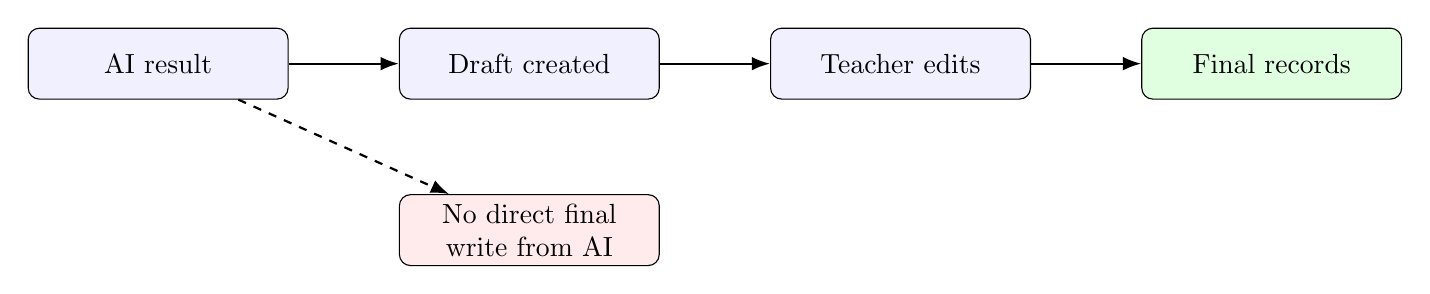
\begin{tikzpicture}[
state/.style={draw, rounded corners, align=center, minimum width=3.3cm, minimum height=0.9cm, fill=blue!6},
good/.style={draw, rounded corners, align=center, minimum width=3.3cm, minimum height=0.9cm, fill=green!12},
bad/.style={draw, rounded corners, align=center, minimum width=3.3cm, minimum height=0.9cm, fill=red!8},
arrow/.style={-Latex, thick}
]
\node[state] (ai) {AI result};
\node[state, right=1.4cm of ai] (draft) {Draft created};
\node[state, right=1.4cm of draft] (edit) {Teacher edits};
\node[good, right=1.4cm of edit] (final) {Final records};
\node[bad, below=1.2cm of draft] (blocked) {No direct final\\write from AI};
\draw[arrow] (ai) -- (draft);
\draw[arrow] (draft) -- (edit);
\draw[arrow] (edit) -- (final);
\draw[arrow, dashed] (ai) -- (blocked);
\end{tikzpicture}
\caption{Attendance draft testing focus}
\label{fig:draft-testing}
\end{figure}

The draft tests check the following outcomes:

\begin{itemize}
\item Draft contains class id, teacher id, present list, absent list and source information.
\item Absentee emails are triggered when the draft is created.
\item Teacher can add a student who was missed by AI.
\item Teacher can remove a student incorrectly marked present.
\item Finalization creates one final attendance entry per roster student for the session.
\item Finalized draft cannot be accidentally finalized again.
\end{itemize}

\section{Security and Privacy Checks}

Security testing for this project focused on preventing accidental exposure. The report, frontend and safe status endpoints must not show MongoDB connection strings, Gmail app passwords or other credentials. OTP values should not appear in production responses. Email delivery logs should store useful metadata and errors without storing secrets.

Document proof also needs careful handling. The teacher should preview files from the application, but the system should avoid encouraging unnecessary downloading. In a production version, file upload should include size limits, type validation and scanning. For this academic implementation, the report documents the expected controls and the application keeps the review workflow inside the class detail context.

\section{Result Analysis}

The implemented project satisfies the core goal of making attendance more transparent and useful. Students can see class-wise attendance and eligibility information rather than only a final percentage. Teachers can run different attendance methods and correct AI results before final submission. Email communication reduces manual reminders. Leave proof connects absence reason to class records.

The main improvement over a traditional register is not only speed; it is feedback. Students receive early absence notifications, exam warnings and leave decision emails. Teachers receive a manageable review workflow. The system also avoids the dangerous assumption that AI output should always be final.

\section{Known Limitations Found During Testing}

Some limitations remain. AI accuracy depends on enrollment quality, lighting, camera angle and image resolution. Email delivery depends on SMTP provider settings and account limits. A real institute deployment would need stronger authentication middleware, role-based authorization on every route, production file storage, stricter upload validation, rate limiting and backups. These limitations do not invalidate the project; they show the difference between a final-year prototype and an institute-wide production rollout.

\section{Testing Conclusion}

Testing shows that the project has a coherent full-stack workflow: registration verifies email, classes can be created and joined, attendance can be captured and reviewed, students can track analytics, teachers can review proof, exams can generate eligibility guidance and emails can notify users. The project is therefore suitable as a final academic project and as a foundation for future production hardening.

\chapter{Deployment, Limitations and Future Scope}
\label{chap:deployment}

This chapter explains how the project can be run, deployed and improved. SAMS is implemented as a multi-service application, so deployment means making the frontend, backend, AI service, database and email provider work together reliably.

\section{Local Development Deployment}

In local development, the project can be started from the repository root. The frontend runs as a React development server, the backend runs as an Express server and the AI service runs with Uvicorn. MongoDB can be provided locally or through Docker.

\begin{table}[H]
\centering
\caption{Local service deployment summary}
\label{tab:local-deployment}
\begin{tabularx}{\textwidth}{p{3cm} p{4cm} X}
\toprule
\textbf{Service} & \textbf{Typical command} & \textbf{Purpose}\\
\midrule
Frontend & \texttt{npm run dev:frontend} & Starts the React interface for browser use.\\
Backend & \texttt{npm run dev:backend} & Starts the REST API and connects to MongoDB.\\
AI service & \texttt{npm run dev:ai} or Uvicorn & Starts FastAPI face recognition endpoints.\\
MongoDB & Docker Compose or local MongoDB & Stores users, classes, attendance and logs.\\
Email SMTP & Configured through backend environment & Sends OTPs and academic notifications.\\
\bottomrule
\end{tabularx}
\end{table}

For a development machine, it is common to run the backend and frontend first, then start the AI service when testing face enrollment or photo attendance. This reduces setup time when working only on dashboards or email templates.

\section{Environment Configuration}

The backend uses environment variables for database, email and AI settings. Sensitive values must never be committed or printed in reports. A safe example is provided in Appendix~\ref{appendix:setup}. In production, values such as database URI and SMTP password should be set through the hosting provider's secret manager.

\begin{table}[H]
\centering
\caption{Important environment categories}
\label{tab:env-categories}
\begin{tabularx}{\textwidth}{p{3.5cm} X}
\toprule
\textbf{Category} & \textbf{Examples of values}\\
\midrule
Server & Port, frontend origin and API base URL.\\
Database & MongoDB connection string and database name.\\
AI gateway & AI service base URL and timeout values.\\
Email & SMTP host, port, sender, username, password and retry settings.\\
OTP & Expiry time and development exposure flag.\\
Model runtime & Face model pack, provider and asset directory.\\
\bottomrule
\end{tabularx}
\end{table}

\section{Production Deployment View}

A production deployment can place the frontend on a static hosting platform, the backend on a Node.js hosting platform, the AI service on a Python-capable host and MongoDB on a managed database service. The backend should be the only service exposed to the frontend. The AI service should be accessible to the backend and protected from direct public misuse when possible.

\begin{figure}[H]
\centering
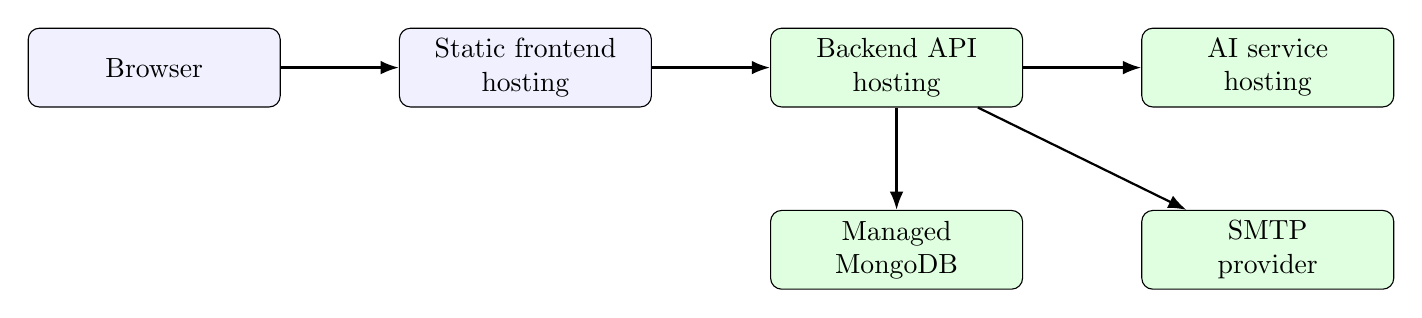
\begin{tikzpicture}[
box/.style={draw, rounded corners, align=center, minimum width=3.2cm, minimum height=1cm, fill=blue!6},
secure/.style={draw, rounded corners, align=center, minimum width=3.2cm, minimum height=1cm, fill=green!12},
arrow/.style={-Latex, thick}
]
\node[box] (user) {Browser};
\node[box, right=1.5cm of user] (front) {Static frontend\\hosting};
\node[secure, right=1.5cm of front] (back) {Backend API\\hosting};
\node[secure, below=1.3cm of back] (db) {Managed\\MongoDB};
\node[secure, right=1.5cm of back] (ai) {AI service\\hosting};
\node[secure, below=1.3cm of ai] (mail) {SMTP\\provider};
\draw[arrow] (user) -- (front);
\draw[arrow] (front) -- (back);
\draw[arrow] (back) -- (db);
\draw[arrow] (back) -- (ai);
\draw[arrow] (back) -- (mail);
\end{tikzpicture}
\caption{Production deployment view}
\label{fig:production-deployment}
\end{figure}

\section{Operational Monitoring}

The project includes health and status concepts that are important for operations. The backend health endpoint can show whether the backend is running and whether dependencies are degraded. The AI service has a readiness endpoint so model loading can be checked separately from process uptime. The email status endpoint can verify SMTP connectivity without revealing credentials.

In a future production system, operational monitoring should include request logs, attendance finalization logs, email bounce tracking, uptime monitoring, database backups and alerts for repeated AI or SMTP failures.

\section{Limitations}

Every project has limitations. Understanding them is important because it prevents unrealistic expectations.

\begin{longtable}{p{3.6cm} p{9.5cm}}
\caption{Current limitations}
\label{tab:limitations}\\
\toprule
\textbf{Area} & \textbf{Limitation}\\
\midrule
\endfirsthead
\toprule
\textbf{Area} & \textbf{Limitation}\\
\midrule
\endhead
AI recognition & Face matching can fail due to poor lighting, blur, occlusion, side angle or incomplete enrollment.\\
Manual review & Teacher review improves reliability but still depends on teacher attention before final submission.\\
Email delivery & Free SMTP or Gmail app passwords may have sending limits and provider-specific security rules.\\
File uploads & A production deployment should add stronger file type validation, file size limits and malware scanning.\\
Authorization & A production institute system should add strict middleware checks for every role and route.\\
Scalability & Large institutes may need queues for AI jobs, background workers and caching.\\
Privacy & Face embeddings and proof documents require formal data retention and consent policies.\\
Network dependency & Real-time email and AI requests depend on network connectivity.\\
\bottomrule
\end{longtable}

\section{Future Scope}

The project can be extended in several directions. Some improvements are technical, while others are academic workflow enhancements.

\begin{table}[H]
\centering
\caption{Future enhancement roadmap}
\label{tab:future-roadmap}
\begin{tabularx}{\textwidth}{p{3cm} p{3cm} X}
\toprule
\textbf{Priority} & \textbf{Enhancement} & \textbf{Expected value}\\
\midrule
High & Strong RBAC middleware & Ensures every route verifies role, identity and class ownership.\\
High & Production file storage & Stores leave documents in object storage with signed access.\\
High & Attendance audit trail & Keeps a history of every draft edit and finalization action.\\
Medium & Background AI queue & Handles large photo attendance jobs without blocking requests.\\
Medium & Parent portal & Gives parents controlled visibility into attendance and alerts.\\
Medium & Reports export & Generates PDF or spreadsheet reports for department records.\\
Medium & Calendar integration & Syncs class schedule and exam dates with external calendars.\\
Low & Mobile app & Improves camera capture, QR scanning and push notifications.\\
Low & Advanced analytics & Predicts future risk patterns and recommends interventions.\\
\bottomrule
\end{tabularx}
\end{table}

\section{Ethical and Privacy Considerations}

Because the project uses face recognition and academic data, ethics must be considered. Students should know why face enrollment is collected and how it is used. The system should store only the data required for attendance. Access to face profiles, attendance data and medical documents should be limited. A production institution should define retention periods and deletion policy.

The human review design is also an ethical choice. AI output is not treated as unquestionable truth. The teacher reviews Today Attendance Data, students receive early absence notices and corrections are possible before final submission. This makes the system more fair than a fully automatic black-box attendance system.

\section{Conclusion}

The \projecttitle{} provides a complete modern attendance workflow. It combines role-based dashboards, class management, AI-assisted attendance, QR and manual attendance, Today Attendance Data, student analytics, leave proof review, exam eligibility planning and email notifications. The project is implemented with a practical full-stack architecture using React, Express, MongoDB and FastAPI.

The most valuable contribution of the project is the combination of automation and review. AI reduces repetitive classroom work, but final attendance remains correctable. Students get useful information instead of only a final number. Teachers get tools to manage attendance, leave and exam eligibility in one place. With stronger production security, file storage and background processing, the system can become a robust institute-level attendance platform.


\appendix
\chapter{Supplementary Material}
\label{appendix:setup}

This appendix gives practical reference material for readers who want to understand the project setup, API surface and data model quickly. All environment examples are sanitized. Real database URLs, SMTP passwords and app passwords must never be written in documentation.

\section{Sanitized Environment Setup}

\subsection{Backend Environment Example}

\begin{verbatim}
NODE_ENV=development
PORT=4000
FRONTEND_ORIGIN=http://localhost:5173
MONGODB_URI=mongodb://localhost:27017/sams

AI_SERVICE_BASE_URL=http://localhost:8000
AI_REQUEST_TIMEOUT_MS=120000
AI_HEALTH_TIMEOUT_MS=10000

EMAIL_ENABLED=true
EMAIL_FROM="SAMS Notifications <your-address@example.com>"
EMAIL_HOST=smtp.gmail.com
EMAIL_PORT=465
EMAIL_SECURE=true
EMAIL_USER=your-address@example.com
EMAIL_PASSWORD=your-app-password
EMAIL_RETRY_COUNT=2
EMAIL_RETRY_DELAY_MS=2000
EMAIL_QUEUE_CONCURRENCY=3
EMAIL_TEST_RECIPIENT=your-test-recipient@example.com
EMAIL_TEST_KEY=change-this-test-key
EMAIL_OTP_EXPIRES_MINUTES=10
EMAIL_EXPOSE_OTP_IN_RESPONSE=false
\end{verbatim}

\subsection{AI Service Environment Example}

\begin{verbatim}
MODEL_DEVICE=cpu
FACE_ANALYSIS_PROVIDERS=CPUExecutionProvider
FACE_ANALYSIS_MODEL_PACK=antelopev2
FACE_ANALYSIS_MODEL_PACKS=antelopev2,buffalo_l
FACE_ANALYSIS_AUTO_DOWNLOAD=true
\end{verbatim}

\section{Common Development Commands}

\begin{table}[H]
\centering
\caption{Common development commands}
\label{tab:dev-commands}
\begin{tabularx}{\textwidth}{p{5.2cm} X}
\toprule
\textbf{Command} & \textbf{Purpose}\\
\midrule
\texttt{npm run dev} & Start multiple project services from the monorepo when configured.\\
\texttt{npm run dev:frontend} & Start the React frontend development server.\\
\texttt{npm run dev:backend} & Start the Express backend server.\\
\texttt{npm run dev:ai} & Start the FastAPI AI service through the project script.\\
\texttt{npm --workspace backend install} & Install backend Node.js dependencies.\\
\texttt{npm --workspace frontend install} & Install frontend Node.js dependencies.\\
\texttt{pip install -r ai-service/requirements.txt} & Install AI service Python dependencies.\\
\texttt{docker compose up} & Start services defined in Docker Compose, including MongoDB when configured.\\
\bottomrule
\end{tabularx}
\end{table}

\section{API Endpoint Summary}

The following table summarizes the major REST endpoints visible from the current backend router. It is not a substitute for generated API documentation, but it helps a reader understand the project scope.

\begin{longtable}{p{2cm} p{6.2cm} p{5.5cm}}
\caption{API endpoint summary}
\label{tab:api-summary}\\
\toprule
\textbf{Method} & \textbf{Endpoint} & \textbf{Purpose}\\
\midrule
\endfirsthead
\toprule
\textbf{Method} & \textbf{Endpoint} & \textbf{Purpose}\\
\midrule
\endhead
GET & \texttt{/api/v1/health} & Backend health and dependency status.\\
GET & \texttt{/api/v1/email/status} & Safe email service status.\\
POST & \texttt{/api/v1/email/verify} & Verify SMTP connection.\\
POST & \texttt{/api/v1/email/test} & Send protected test email.\\
GET & \texttt{/api/v1/attendance/summary} & General attendance summary.\\
POST & \texttt{/api/v1/attendance/verify} & Attendance verification endpoint.\\
POST & \texttt{/api/v1/auth/signup} & Register user and start verification.\\
POST & \texttt{/api/v1/auth/login} & Log in user.\\
POST & \texttt{/api/v1/auth/verify-email} & Verify email OTP.\\
POST & \texttt{/api/v1/auth/resend-verification} & Resend signup verification OTP.\\
POST & \texttt{/api/v1/auth/password-reset/request} & Request password reset OTP.\\
POST & \texttt{/api/v1/auth/password-reset/confirm} & Confirm password reset.\\
POST & \texttt{/api/v1/users/:role/:userId/email-otp} & Send OTP for profile email update.\\
PATCH & \texttt{/api/v1/users/:role/:userId/profile} & Update user profile after validation.\\
GET & \texttt{/api/v1/classes/:classId/assignments} & List class assignments.\\
GET & \texttt{/api/v1/classes/:classId/discussion} & List class discussion messages.\\
POST & \texttt{/api/v1/classes/:classId/discussion} & Post a class discussion message.\\
POST & \texttt{/api/v1/classes/:classId/discussion/:messageId/replies} & Add reply to discussion message.\\
POST & \texttt{/api/v1/classes/:classId/discussion/:messageId/reactions} & React to a discussion message.\\
GET & \texttt{/api/v1/students/:userId/dashboard} & Load student dashboard summary.\\
POST & \texttt{/api/v1/students/:studentId/classes/join} & Student joins a class.\\
POST & \texttt{/api/v1/students/:studentId/classes/:classId/assignments/:assignmentId/submissions} & Submit assignment work.\\
POST & \texttt{/api/v1/students/:studentId/classes/:classId/leave-requests} & Submit leave or medical proof.\\
GET & \texttt{/api/v1/students/:studentId/face-profile} & Load face enrollment profile state.\\
POST & \texttt{/api/v1/students/:studentId/face-profile/enroll} & Enroll student face profile.\\
GET & \texttt{/api/v1/teachers/:userId/dashboard} & Load teacher dashboard summary.\\
POST & \texttt{/api/v1/teachers/:teacherId/classes} & Teacher creates a class.\\
POST & \texttt{/api/v1/teachers/:teacherId/classes/:classId/assignments} & Teacher creates assignment.\\
PATCH & \texttt{/api/v1/teachers/:teacherId/classes/:classId/exam} & Set exam date and required percentage.\\
GET & \texttt{/api/v1/teachers/:teacherId/classes/:classId} & Load teacher class detail.\\
POST & \texttt{/api/v1/teachers/:teacherId/classes/:classId/students} & Add student to class roster.\\
PATCH & \texttt{/api/v1/teachers/:teacherId/classes/:classId/students/:studentId} & Update roster student.\\
DELETE & \texttt{/api/v1/teachers/:teacherId/classes/:classId/students/:studentId} & Remove roster student.\\
POST & \texttt{/api/v1/teachers/:teacherId/classes/:classId/attendance/manual} & Submit manual attendance.\\
POST & \texttt{/api/v1/teachers/:teacherId/classes/:classId/cancel-today} & Cancel today's class.\\
POST & \texttt{/api/v1/teachers/:teacherId/classes/:classId/attendance/qr-session} & Create QR attendance session.\\
POST & \texttt{/api/v1/students/attendance/qr-scan} & Student marks attendance through QR scan.\\
POST & \texttt{/api/v1/teachers/:teacherId/classes/:classId/attendance/session} & Process photo attendance and create draft.\\
PATCH & \texttt{/api/v1/teachers/:teacherId/classes/:classId/attendance/today-draft/:draftId} & Update Today Attendance Data draft.\\
POST & \texttt{/api/v1/teachers/:teacherId/classes/:classId/attendance/today-draft/:draftId/finalize} & Finalize Today Attendance Data draft.\\
POST & \texttt{/api/v1/teachers/:teacherId/classes/:classId/attendance/finalize} & Finalize attendance records directly.\\
PATCH & \texttt{/api/v1/teachers/:teacherId/classes/:classId/leave-requests/:requestId} & Approve or reject leave request.\\
\bottomrule
\end{longtable}

\section{Model and Collection Reference}

\begin{longtable}{p{3.7cm} p{9.5cm}}
\caption{Model reference}
\label{tab:model-reference}\\
\toprule
\textbf{Model} & \textbf{Main fields and meaning}\\
\midrule
\endfirsthead
\toprule
\textbf{Model} & \textbf{Main fields and meaning}\\
\midrule
\endhead
User & user id, role, name, email, parent email, email verified flag and profile fields.\\
EmailOtp & email, purpose, OTP hash or value metadata, expiry and used state.\\
Classroom & class id, teacher id, subject name, subject code, section, room, semester and schedule slots.\\
ClassMembership & class id, student id, membership state and timestamps.\\
AttendanceRecord & class id, student id, student name, status, source, recorded date and notes.\\
AttendanceDraft & class id, teacher id, draft records, source, created time, finalize time and final status.\\
QrAttendanceSession & class id, session code, expiry, active state and scan information.\\
FaceProfile & student id, enrollment state and face recognition metadata.\\
LeaveRequest & class id, student id, absence date, reason, type, attachments, status and teacher note.\\
ClassExam & class id, exam title, exam date, required attendance percentage and notes.\\
EmailDeliveryLog & recipient, template name, notification key, status, attempts and error summary.\\
ClassAssignment & class id, teacher id, title, description, due date and attachment metadata.\\
ClassAssignmentSubmission & assignment id, class id, student id, submitted content and status.\\
ClassDiscussionMessage & class id, author, message, replies, reactions and timestamps.\\
\bottomrule
\end{longtable}

\section{Sample Email Template Content}

The exact design of email templates can be changed, but every template should include clear subject, greeting, dynamic class or account information and a short action line. The following examples are intentionally generic.

\begin{table}[H]
\centering
\caption{Sample email subjects}
\label{tab:email-subjects}
\begin{tabularx}{\textwidth}{p{4cm} X}
\toprule
\textbf{Event} & \textbf{Sample subject line}\\
\midrule
Signup verification & Verify your SAMS account\\
Welcome message & Welcome to MarkIn / SAMS\\
Password reset & Reset your SAMS password\\
Profile email verification & Confirm your new profile email\\
Leave approved & Your leave request has been approved\\
Leave rejected & Your leave request has been reviewed\\
Exam attendance warning & Attendance warning for upcoming exam\\
Absent notification & You were marked absent today\\
Class cancellation & Class cancelled or rescheduled\\
\bottomrule
\end{tabularx}
\end{table}

\section{Report Figure Inventory}

\begin{table}[H]
\centering
\caption{Important diagrams included in the report}
\label{tab:figure-inventory}
\begin{tabularx}{\textwidth}{p{4cm} X}
\toprule
\textbf{Diagram} & \textbf{Purpose}\\
\midrule
Overall architecture & Shows frontend, backend, AI service, database and email relationship.\\
Service communication & Explains API calls and data flow between services.\\
Entity relationship & Explains MongoDB collections and relationships.\\
Today Attendance Data flow & Shows draft creation, absentee alert, correction and finalization.\\
Email notification flow & Shows event, template, queue, SMTP and delivery log.\\
Student dashboard flow & Shows dashboard to class, notification and tool pages.\\
Teacher attendance flow & Shows manual, QR and AI photo attendance routes.\\
Leave proof flow & Shows upload, preview, approve or reject and notification.\\
Deployment view & Shows production hosting arrangement.\\
\bottomrule
\end{tabularx}
\end{table}

\section{Glossary}

\begin{longtable}{p{3.3cm} p{10cm}}
\caption{Glossary}
\label{tab:glossary}\\
\toprule
\textbf{Term} & \textbf{Meaning}\\
\midrule
\endfirsthead
\toprule
\textbf{Term} & \textbf{Meaning}\\
\midrule
\endhead
SAMS & Smart Attendance Management System.\\
MarkIn & Product name used for the SAMS application.\\
Attendance draft & Temporary attendance data created before final submission.\\
Today Attendance Data & Teacher review section for current draft attendance.\\
Face enrollment & Process where a student registers face data for AI attendance.\\
OTP & One-time password sent by email for verification or password recovery.\\
Eligibility percentage & Minimum attendance required to appear in an exam.\\
Roster & List of students enrolled in a class.\\
SMTP & Standard protocol used for sending email through a mail provider.\\
Mongoose & MongoDB object modelling library used in the backend.\\
FastAPI & Python framework used for the AI service.\\
\bottomrule
\end{longtable}


\begin{thebibliography}{99}
\bibitem{mern}
MongoDB, Express, React and Node.js documentation, ``MERN stack application development,'' online documentation, accessed May 2026.

\bibitem{fastapi}
FastAPI documentation, ``FastAPI framework, high performance APIs with Python,'' online documentation, accessed May 2026.

\bibitem{insightface}
InsightFace project documentation, ``2D and 3D face analysis toolkit,'' online documentation, accessed May 2026.

\bibitem{arcface}
J. Deng, J. Guo, N. Xue and S. Zafeiriou, ``ArcFace: Additive Angular Margin Loss for Deep Face Recognition,'' in \textit{Proceedings of the IEEE/CVF Conference on Computer Vision and Pattern Recognition}, 2019.

\bibitem{scrfd}
D. Guo et al., ``Sample and Computation Redistribution for Efficient Face Detection,'' SCRFD face detection model documentation and associated research resources, accessed May 2026.

\bibitem{nodemailer}
Nodemailer documentation, ``Send emails from Node.js,'' online documentation, accessed May 2026.

\bibitem{mongodb}
MongoDB documentation, ``Document data model, indexing and query operations,'' online documentation, accessed May 2026.

\bibitem{react}
React documentation, ``Building user interfaces with components,'' online documentation, accessed May 2026.

\bibitem{samsrepo}
Project source repository documentation, \textit{Smart Attendance Management System README, architecture notes and email notification notes}, local project documentation, 2026.
\end{thebibliography}

\end{document}
